\documentclass[letterpaper,12pt]{article}
\usepackage[utf8]{inputenc}

\usepackage[T1]{fontenc}
\usepackage{charter} %%%font


\usepackage[spanish]{babel}
\usepackage{pdfpages}
\usepackage{geometry}
\usepackage{amsmath}
\usepackage{float}
\usepackage{graphicx}
\usepackage{subcaption}
\usepackage{amssymb}
\usepackage{adjustbox}
\usepackage{wrapfig} %%imagen envuelta por un texto
\usepackage{xcolor}
\usepackage{fancyhdr}
\usepackage{tabularx} %%TABLAS OH YEAH


\thispagestyle{empty}
\title{\textcolor[rgb]{0.3,0.4,0.9}{\textbf{"El administrador como lider"}}} 
\author{\textbf{Equipo H.A.D - Gestión Empresarial} \\ Martínez Schleske Alan \\ López Castillo Haziel \\ Lara Xocuis Martha Denisse}
\date{30 de Agosto de 2023}


\geometry{top=2cm, bottom=2cm, left=2cm, right= 2cm} %%margen
\graphicspath{{images/}}

\begin{document}
\maketitle
\thispagestyle{empty}
\newpage
\thispagestyle{empty}
\tableofcontents %%%%%%%%%%%%%%%%%%%%%%
\newpage
\listoffigures
\thispagestyle{empty}
\newpage
\setcounter{page}{1}
\pagestyle{headings}

\begin{sloppypar}
\section*{\title{\textcolor[rgb]{0.4,0.4,0.9}{\textbf{Introducción}}}}
La comprensión de una empresa, su misión y objetivos determinados es realmente fundamental a la hora de enfocarnos en la gestión y la administración de dicha empresa, el objeto de la aplicación tanto de la gestión como de la administración son los organismos sociales productivos, entre los que se encuentran sobre todo las empresas productivas, tanto micro como pequeñas, medianas y grandes, además de otras formas de organización de producción. 

Dentro de este proyecto de investigación se encuentra un minucioso trabajo de análisis sobre \textbf{"Faurecia"}, una empresa de fabricación de componentes automovilísticos, se impartirá tanto su historia, sedes, fortalezas industriales, adquisisiones, ambiciones y grupos combinados, en base a esto nos enfocamos más sobre una amplia \textit{estructura} de la empresa y poder entenderla como una \textit{unidad económico-social}, es decir, sabiendo que una empresa produce bienes y servicios necesarios para satisfacer necesidades sociales, podemos adentrarnos sobre la complejidad de su competencia laboral, su sistema, objetivos, entorno y administración; este último punto es muy importante por la gran profundidad que conlleva sobre si mismo, si pensamos en administrar algo llegamos a un nivel de planteamiento clave donde se empiezan a tomar en cuenta factores más a largo plazo y, por lógica, siguiendo los conceptos de administración, el administrador será quien ejecute actividades administrativas, es decir, \textbf{alguien que dirige personas y emplea recursos para conseguir objetivos.}
\vspace{0.3cm}\\ 
Es de vital importancia tomar en cuenta la organización interna de una empresa, no solo enfocarse en un \textit{"lider"} sino también a sus empleados y sus cargos, es necesario que todas las partes funcionen para poder alcanzar el mayor de los beneficios deseados, es por eso que se comparten distintos conceptos dentro de este trabajo con el objetivo de una visión más amplia sobre lo que rige una empresa. Se introducirá, incluso, nuestro propio perfil de un administrador apto para las necesidades globales de una organización administrativa. Claro está que se tomarán en cuenta las características (aptitudes, conocimientos, importantes reglamentos legales, entre otros) con el fin de indagar dentro de una base empresarial.

%%%%%%%%%%%%%%%%%%%%%%%%%%%%%%
\newpage
\section{\textcolor[rgb]{0.4,0.4,0.9}{FAURECIA}}
\subsection{\textcolor[rgb]{0.9,0.3,0.3}{¿Qué es?}}
Faurecia es un holding dedicado a la fabricación y suministro de componentes de automoción, inició su sede en Nanterre, Francia y --actualmente-- tiene a Patrik Koller como ejecutivo principal, cuentan con más de 157,000 empleados dentro de la empresa. 

Fundada en 1997, Faurecia ha crecido hasta convertirse en un jugador importante en la industria automotriz a nivel mundial. Con 266 sitios industriales, 39 centros de I+D y 114,000 empleados en 35 países, Faurecia es un líder global en sus cuatro áreas de negocios: \textbf{Asientos, Interiores, Clarion Electronics y Movilidad Limpia.} 
\vspace{0.3cm}\\ 
En febrero de 2022, \textit{Faurecia y HELLA} presentaron \textbf{FORVIA}, el nombre del recientemente Grupo combinado, tras la finalización exitosa de la adquisición de una participación mayoritaria en HELLA por parte de Faurecia el 31 de enero de 2022. La sólida oferta tecnológica del Grupo proporciona a los fabricantes de automóviles soluciones para la Cabina del Futuro y la Movilidad Sustentable. En 2020, el Grupo registró una facturación total de 14,700 millones de euros. \textbf{\textit{(Anexo \ref{fig: 1 })}}

\subsubsection{¿Qué hace FAURECIA?}
Está dedicada a la fabricación y suministro de componentes de automoción y está especializada en la producción de piezas para automóviles: asientos, paneles de instrumentos, paneles de puertas, tecnologías para reducir las emisiones de $CO_2$ --la empresa también está apostando fuerte por el hidrógeno--, tiene previsto construir una planta de producción de tanques de hidrógeno.

Opera a través de los siguientes segmentos de negocio: \textbf{Faurecia Automotive Seating, Faurecia Emissions Control Technologies, Faurecia Interior Systems y Faurecia Automotive Exteriors.}

\begin{enumerate}
    \item \textbf{Faurecia Automotive Seating:} se dedica al diseño de asientos para vehículos, la fabricación de armazones de asientos y mecanismos de ajuste, y el montaje de unidades de asiento completas. 
    \item \textbf{Faurecia Emissions Control Technologies :} se dedica a la fabricación y diseño de sistemas de escape
    \item \textbf{Faurecia Interior Systems:} fabrica y diseña paneles de instrumentos, paneles y módulos de puertas y componentes acústicos
    \item \textbf{Faurecia Automotive Exteriors: }se dedica al diseño y fabricación de frontales y módulos de seguridad.
\end{enumerate}
\newpage
\subsubsection{Faurecia México}
Faurecia México es una empresa líder en la fabricación de soluciones y tecnologías para la industria automotriz. Inició sus operaciones en el país en 1997 estableciéndose en el Parque Industrial FINSA de la ciudad de Puebla como Sommer Allibert Industries para la fabricación de Interiores. Desde entonces, Faurecia ha crecido y extendido sus zonas de producción hasta abarcar diferentes estados de la República como Puebla, Querétaro, Guanajuato, San Luis Potosí, Coahuila y Sonora.

Se ha convertido en pieza clave para la industria automotriz gracias a su firme compromiso con la digitalización de procesos, en los que cada planta puede dar seguimiento a su producción en tiempo real, a la par de analizar la eficiencia y planes de acción a detalle. \textbf{\textit{(Anexo \ref{fig: 2})}}

\subsubsection{Historia}
En 1914, Bertrand Faure \textbf{\textit{(Anexo \ref{fig: 3})}} abrió su primer taller en Levallois-Perret, a las afueras de París, fabricando asientos para tranvías y el metro de París. Desde entonces, Faurecia ha crecido hasta convertirse en uno de los diez principales proveedores mundiales de automoción, trabajando para dar forma a la próxima generación de movilidad en cada momento.

Faurecia, tal y como la conocemos hoy en día, se formó con la adquisición de Bertrand Faure por parte de ECIA, propiedad de PSA, para crear una empresa mundial. En 2021, con la fusión de PSA y FCA y la creación de Stellantis, comenzó un nuevo capítulo en la historia de Faurecia.
\begin{center}
    \textbf{\textit{A continuación una línea de tiempo más detallada sobre la historia de esta empresa:}}
\end{center}
\begin{itemize} %%linea del tiempo
    \item 1914: Bertrand Faure abre un taller para fabricar asientos para tranvías y trenes metropolitanos.
    \item 1929: Faure adquiere la patente del muelle Epéda y comienza comienza la producción de sistemas de asientos para el mercado del automóvil, esta fue la fecha en que fue fundada. 
    \item 1945: Peugeot inicia la producción de componentes de automoción, bicicletas y motocicletas a través de las filiales Aciers et Outillage Peugeot y Peugeot Cycles.
    \item 1987:  Aciers et Outillage Peugeot y Peugeot Cycles se fusionan para formar ECIA; Faure adquiere Delsey y Luchaire.
    
    ECIA había firmado contratos con otros fabricantes de automóviles, como Volkswagen y Renault, que representaron el 18\% y el 11\%, respectivamente, de los ingresos de ECIA ese año, frente al 60\% de PSA Peugeot-Citroën. Otros clientes eran Daimler Benz, Opel Honda y Mitsubishi. Para entonces, las ventas de la empresa habían superado los 1.600 millones de euros, el doble que en 1987. El porcentaje de componentes de automoción en los ingresos totales de ECIA se había más que triplicado durante este tiempo.

    \item 1988: Bertrand Faure es adquirido en una LBO respaldada por Michelin, Michel Thierry, Peugeot y otros para bloquear un intento de adquisición por parte de Valeo.
    \item 1991: Faure adquiere Rentrop en Alemania.
    \item 1996:  la complejidad del paquete de adquisición de Faure se volvió en contra de la empresa, cuando Michel Thierry decidió vender su participación del 16,6\% en Faure a ECIA. Este movimiento precipitó las conversaciones entre las dos empresas, que desembocaron en una oferta de adquisición a gran escala de Faure por parte de ECIA a finales de 1997. 
    \item 1998: Faure acuerda ser adquirida por ECIA, formando \textbf{Faurecia}. A fusión, completada en 1998, creó un nuevo gigante francés y europeo, Faurecia. Aunque Faurecia seguía estando controlada por PSA Peugeot-Citroën, que poseía más del 70\% de sus acciones y seguía siendo su principal cliente, la nueva empresa se constituyó como una compañía de funcionamiento independiente.
    \item 1999: Faurecia adquiere AP Automotive Systems en Estados Unidos.
    \item 2001: Faurecia adquirió la división de automoción de Sommer Allibert, formando así el principal proveedor europeo de componentes de automoción.
    \item 2003: Faurecia consigue un contrato de 2.000 millones de dólares para la producción de componentes de cabina para Chrysler en Estados Unidos.
    \item 2004: Faurecia avanzó en su esfuerzo por diversificar su base de clientes. En 2005, la empresa había firmado contratos con un número cada vez mayor de fabricantes de automóviles, entre ellos Volvo, DaimlerChrysler, Saab y BMW. A mediados de la década, Faurecia también se convirtió en uno de los principales proveedores de General Motors. En octubre de 2004, la empresa inició la producción de cabinas para el nuevo Pontiac G6, imponiéndose a los favoritos Johnson Controls y Lear por el contrato. Más tarde, en noviembre de 2004, Faurecia recibió un contrato de casi 2.000 millones de dólares para fabricar paneles de instrumentos, paneles de puertas, consolas centrales y otros componentes para las cabinas de los automóviles estadounidenses de Chrysler. Faurecia se había consolidado como una fuerza clara y creciente en el mercado mundial de componentes de automoción.
    \item 2005: En su lugar, Faurecia empezó a ampliar su presencia internacional, abriendo nuevas plantas en Brasil y Polonia en 1998. Al año siguiente, la empresa se centró en Norteamérica y adquirió AP Automotive Systems (APAS), el tercer productor de sistemas de escape del mercado. La presencia de Faurecia en Norteamérica también se vio impulsada ese año, cuando se le adjudicó un importante contrato de producción para General Motors. La empresa no tardó en ampliar su capacidad de producción en Norteamérica, abriendo o adquiriendo fábricas hasta alcanzar casi 30 instalaciones en ese mercado en 2005.
    \item 2021:con la fusión de PSA y FCA y la creación de Stellantis, comenzó un nuevo capítulo en la historia de Faurecia. Groupe PSA, la multinacional francesa que producía las marcas Peugeot, Citroën, DS, Opel y Vauxhall, era accionista mayoritario de Faurecia. Cuando Groupe PSA se fusionó con Fiat Chrysler para formar Stellantis, Faurecia se independizó y adquirió una participación de control en HELLA
\end{itemize}
\begin{center}
    \textbf{\textit{Para una mejor visualización, se anexa el gráfico resumido de la línea del tiempo en la siguiente página.}}
\end{center}
\newpage
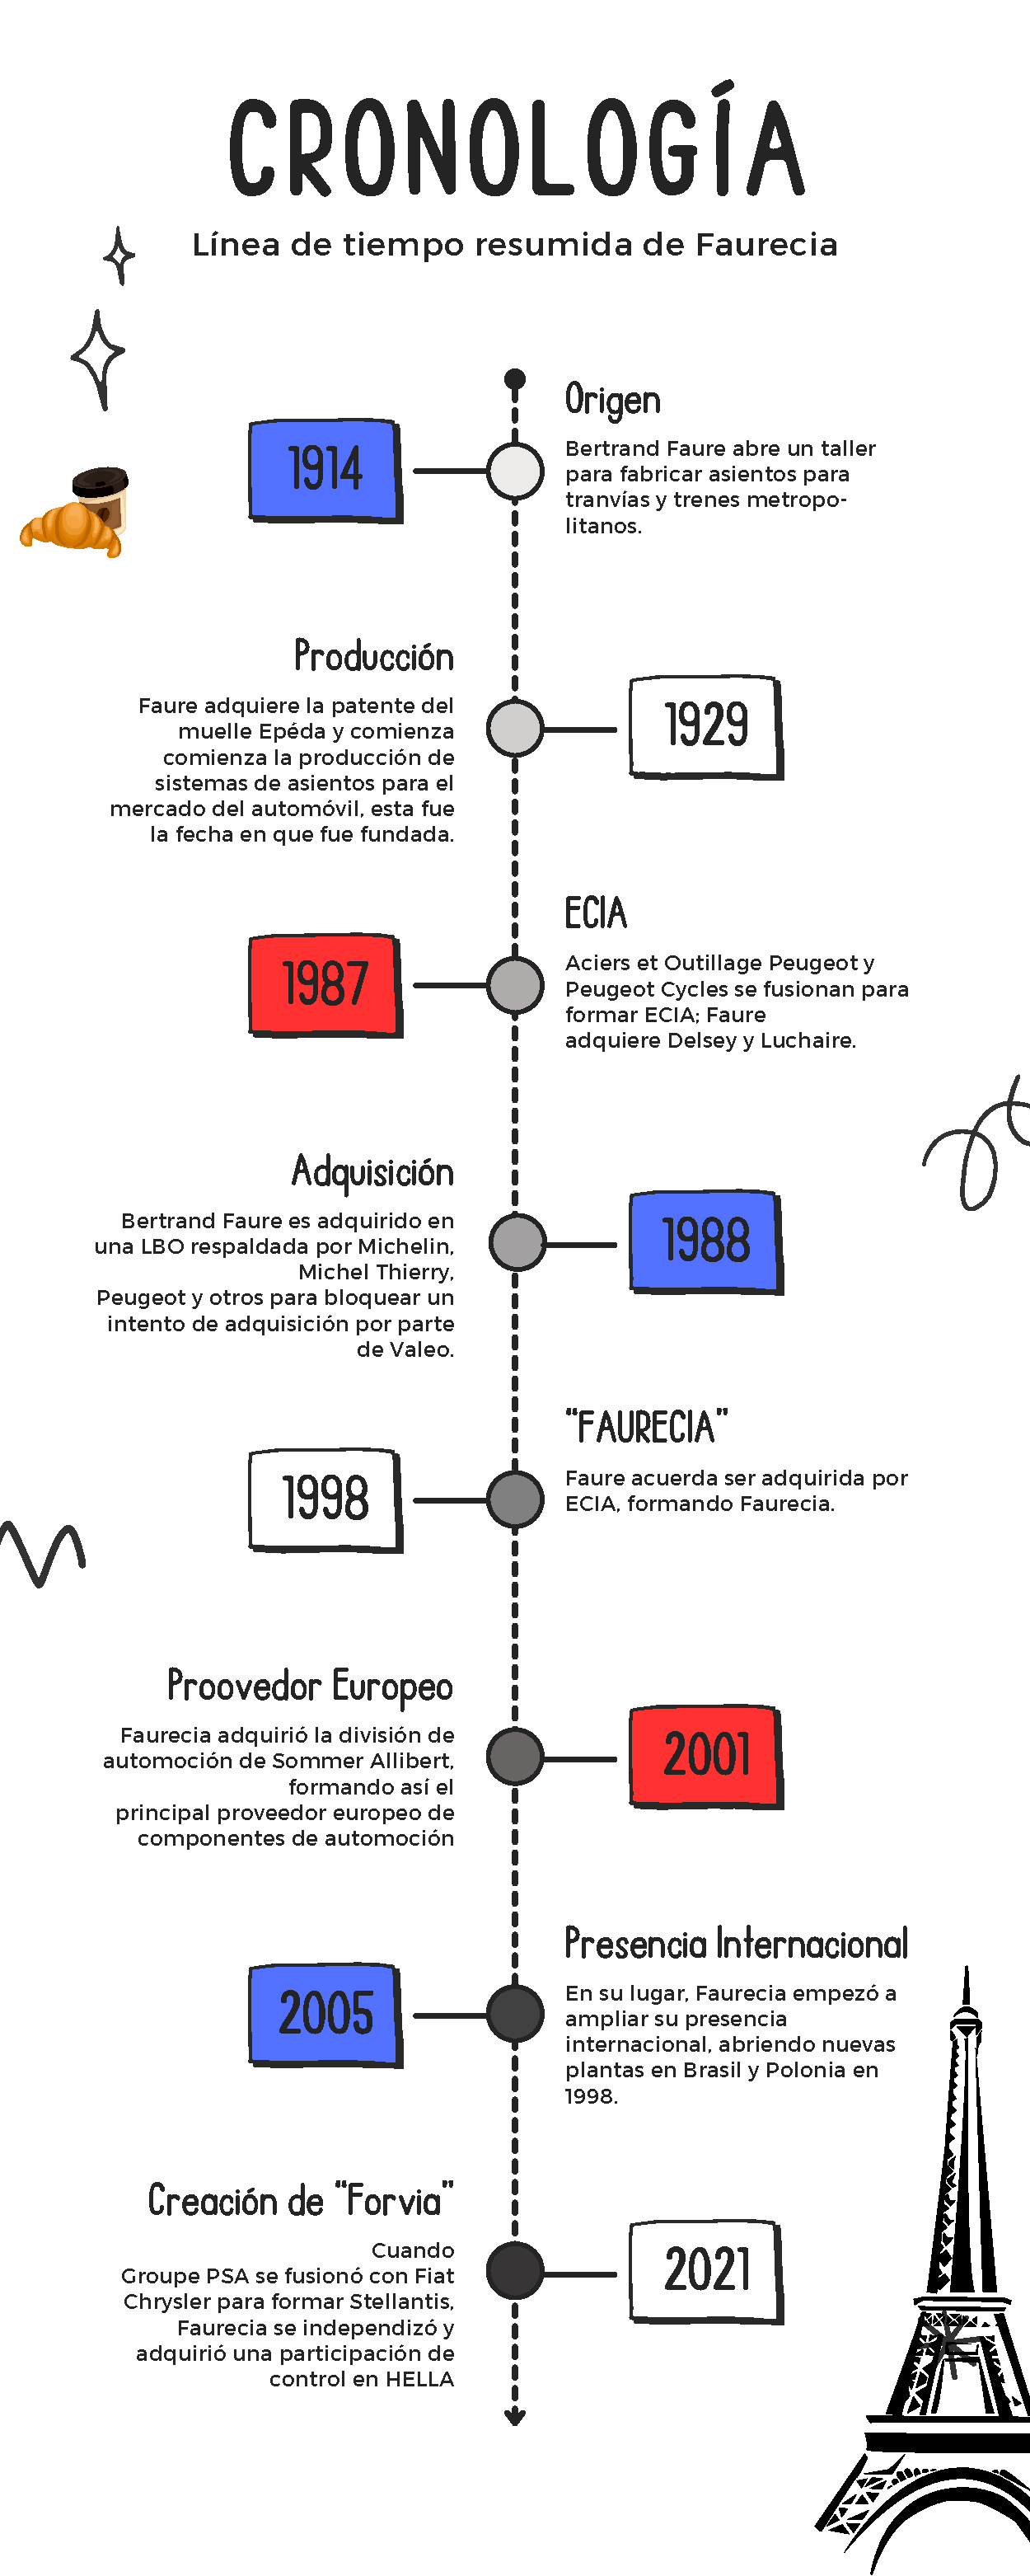
\includepdf[pages=-]{lineapdf.pdf}


\newpage
\subsection{\textcolor[rgb]{0.9,0.3,0.3}{Acerca de FORVIA}}
\subsubsection{¿Qué es?}
FORVIA\textbf{ \textit{(Anexo \ref{fig:4})}} comprende la tecnología complementaria y las fortalezas industriales de Faurecia y HELLA. Con más de 300 sitios industriales y 77 centros de I+D, 150,000 personas, incluidos más de 35,000 ingenieros en más de 40 países, FORVIA ofrece un enfoque único e integral para los desafíos automotrices de hoy y de mañana. Compuesto por 6 grupos de negocio con 24 líneas de productos y una sólida cartera de propiedad intelectual de más de 14,000 patentes, Forvia se enfoca en convertirse en el socio de innovación e integración preferido para los OEM en todo el mundo. FORVIA pretende ser un agente de cambio comprometido con prever y hacer realidad la transformación de la movilidad.
\subsubsection{HELLA}
Esta empresa alemana es líder mundial en tecnología de iluminación para automóviles. También está especializada en componentes electrónicos. En 2021, el proveedor automovilístico generó unas ventas de 6.500 millones de euros y cuenta con algo más de 36.000 empleados en todo el mundo.

Fundada en Alemania en 1899, \textbf{HELLA} es uno de los principales proveedores de tecnología punta en iluminación y electrónica para vehículos. Al mismo tiempo, la empresa cubre una amplia cartera de servicios y productos para el negocio de recambios y talleres, así como para fabricantes de diversos vehículos especiales, por ejemplo de los sectores de la construcción, la agricultura o el transporte. HELLA es una empresa que cotiza en bolsa y que estuvo participada mayoritariamente por las familias Hueck y Roepke antes de que Faurecia se convirtiera en accionista mayoritario.

\subsubsection{¿Qué significa la adquisición con HELLA?}
Faurecia ha adquirido en total alrededor del 79,5\% de las acciones de Hella. Con la adquisición de su homólogo alemán, Faurecia cambia también su nombre por el de \textbf{Forvia}. Con unas ventas combinadas de más de 20.000 millones de euros y 155.000 empleados, Forvia se convierte en el séptimo proveedor mundial de la industria automovilística.

Los dos grupos seguirán funcionando como dos entidades jurídicas independientes, pero operarán en determinados sectores. No obstante, se comunicarán bajo el nombre de Forvia, utilizado como \textbf{"nombre paraguas".}

\subsubsection{Ambiciones de FORVIA}
El grupo piensa a lo grande.\textit{'Uno de cada dos coches fabricados en el mundo estará equipado con productos Forvia'}, dijo Patrick Koller, Director General de Faurecia. Con la compra de Hella, la empresa francesa adquiere tecnologías, sobre todo en iluminación, para seguir desarrollándose en el mercado del coche eléctrico. \textit{'En 2025, el volumen de negocios de la electrónica ascenderá a 7.000 millones de euros'}, afirma Patrick Koller.

La empresa también apuesta fuerte por su \textbf{'cabina del futuro'}, un salpicadero inmersivo y conectado para vehículos. \textit{'Como Forvia, estamos dando forma a una movilidad segura, sostenible, tecnológica e individualizada, hoy y para las generaciones futuras'}, continúa. El nuevo gigante automovilístico aspira a facturar 33.000 millones de euros en 2025.

Al unir Faurecia y HELLA viene la creación de FORVIA, se ha creado un nuevo líder global en tecnología de automoción con la experiencia y la pasión para el futuro de la movilidad, en línea con las tendencias que están transformando la industria del automóvil : electrificación, conducción automatizada y autónoma, y experiencias personalizadas a bordo.
\vspace{0.3cm}\\ 
La visión y la estrategia de FORVIA encarnan un grupo comprometido a impulsar el cambio en la movilidad la tecnología complementaria y las fortalezas industriales de Faurecia y HELLA. Combinadas, estas dos compañías tienen una amplia cartera de soluciones de automoción con posiciones de liderazgo en tecnologías clave y segmentos de rápido crecimiento, creando las condiciones ideales para un crecimiento sostenible y rentable. 

\section{\textcolor[rgb]{0.4,0.4,0.9}{Competencias y habilidades del Administrador}}
\subsection{Conceptos clave}
Se define como competencia la capacidad de una persona para colocar en práctica un conjunto de conocimientos, habilidades y actitudes en el desempeño de una actividad laboral.

Estas son un rasgo entre las características individuales y las cualidades requeridas para un cargo. Para un individuo calificado, la competencia se mide por medio del saber hacer \textit{(cuantitativamente)} y del saber ser \textit{(cualitativamente).} Una organización debe tener buenos líderes que lleven a su equipo de trabajo por el mejor camino logrando con proactividad e iniciativa los mejores resultados, de acuerdo a los objetivos, misión y visión que tiene la organización.
\vspace{0.3cm}\\ 
Un buen líder debe prepararse para desarrollar competencias y habilidades para gestionar una organización; siempre debe estar focalizado, saber para dónde va, cómo lo logrará, con qué medios, por qué motivo, con quién cuenta para lograrlo, cuándo. Esto se logra con el fin de que el líder no pierda sus esfuerzos y cumplir de manera exitosa todo lo emprendido.
\subsubsection{El administrador como lider}
El \textbf{Administrador} debe tener la habilidad gerencial de comprender primero y luego ser comprendido, creando relaciones humanas afectivas que tiendan al ganar–ganar. El trabajo de un administrador se basa en la planeación, organización, integración y la medición.

Los gerentes actuales les gusta lo que hacen, sienten empatía con los demás, cada vez se preparan de mejor manera para desarrollar las capacidades necesarias para tener un buen liderazgo frente a sus equipos de trabajo, administrar con empatía, tomar decisiones acertadas, resolver con éxito los problemas y conflictos, capacidad para trabajar en equipo, saber correr riesgos, innovar, crear, empatizar con las demás personas, entre otros factores que hacen posible el logro de metas y objetivos esperados por la organización basados en la misión y visión. 
\vspace{0.3cm}\\ 
Deben desarrollar habilidades, disciplinas y conocimientos que les permitan llevar a sus equipos de trabajo a la cima, posicionándose en los principales lugares con calidad, logrando los resultados que la organización requiere y un verdadero cambio organizacional. 
\newpage
\subsection{El administrador}
\textit{La profesión de administración es muy variada}, pero depende del nivel en que él se sitúe. Además, deberá vivir con la rutina y con la incertidumbre diaria de las actividades de su departamento o división; incluso, con el proceso decisorio en el nivel institucional, orientado hacia un ambiente externo que la empresa pretende servir.
\vspace{0.3cm}\\ 
\textbf{Es necesario distinguir algunos conceptos:}
\begin{itemize}
    \item \textbf{Eficacia}: conseguir los objetivos trazados, sin importar los medios o recursos empleados.
    \item \textbf{Eficiencia}: conseguir resultados, utilizando la menor cantidad de recursos disponibles.
    \item \textbf{Eficacia = eficacia + eficiencia}: conseguir los objetivos trazados, utilizando la menor cantidad de recursos disponibles 
\end{itemize}
\subsubsection{Nivel jerárquico y responsabilidades}
Las \textit{funciones} del administrador están definidas por algunas características como los \textbf{niveles jerárquicos} en los cuales se desenvuelve en los puestos que desempeña y la responsabilidad que juega en los objetivos y estrategias de la organización.
\vspace{0.3cm}\\
Algunas funciones básicas del administrador y que forman parte del trabajo rutinario de la organización están definidas de la siguiente manera: \textit{'El administrador define estrategias, diagnostica situaciones, mide los recursos, planea su integración, soluciona problemas y genera innovaciones y competitividad'}. Dentro de la agenda organizacional de las funciones del administrador, encontramos con calidad y responsabilidad social. 
\vspace{0.3cm}\\ 
Las \textbf{responsabilidades generales }que debe de tener un administrador son las siguientes:

\begin{itemize}
    \item \textbf{Cumplimiento de metas}: El administrador es el principal respnsable de que se cumplan las metas organizacionales.
    \item \textbf{Orientador}: El administrador imprime dirección y rumbo a las organizaciones.
    \item \textbf{Motor de las organizaciones}: El administrador es la fuerza y el poder de las organizaciones.
    \item \textbf{Formador de capacidades}: El administrador desarrolla capacidades entre sus colaboradores y busca la calidad y competitividad de sus empresas en un entorno globalizado.
    \item \textbf{Optimizador de recursos}: El administrador es un optimizador de los recursos materiales, técnicos y humanos.
\end{itemize}
\newpage
\subsection{Niveles administrativos generales}
No todas las decisiones que se toman al realizar actividades administrativas tienen la misma importancia, dificultad o responsabilidad para quien las realiza. Por tal motivo, es bueno tener una clasificación de los niveles en los cuales puede estar operando un administrador. \textit{(Anexo \ref{fig:5})}
\vspace{0.3cm}\\ 
\textbf{Nivel estratégico:} El nivel estratégico es la administración del nivel superior (Alta Dirección), que tiene el mayor poder y lleva la responsabilidad total de una empresa.
\vspace{0.3cm}\\ 
\textbf{Nivel táctico:} El nivel táctico es el conjunto de gerentes, jefes de línea u oficina, que reportan a la administración del nivel más alto el funcionamiento detallado de la empresa; además de desarrollar planes para implementar las metas generales establecidas por la Alta Dirección.
\vspace{0.3cm}\\ 
\textbf{Nivel operativo:} El nivel operativo está constituido por el personal operativo y por quienes supervisan directamente sus operaciones (supervisores, coordinadores de turno, capataces, etc.)

\subsection{Organigrama}
\begin{figure}[H]
    \centering 
    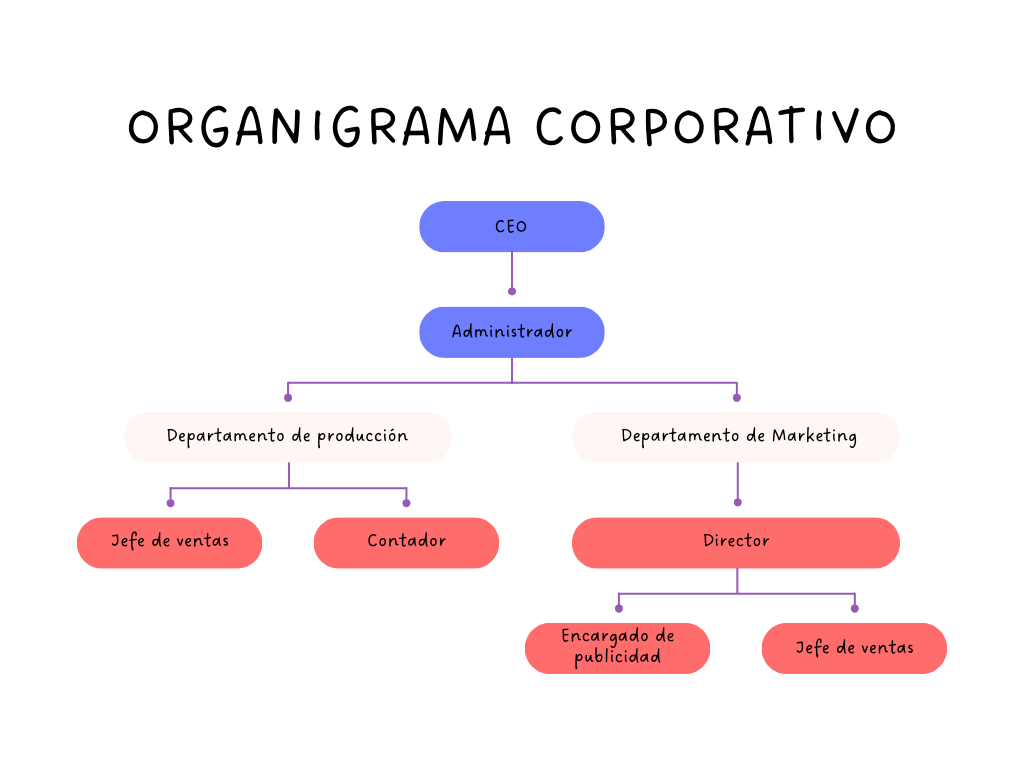
\includegraphics[width=0.9\textwidth]{images/organigramaaaa2.png}
\end{figure}
Explicando un poco del gráfico y su estructura, empezamos el primer nivel(CEO) que se encarga de tomar las decisiones importantes; son los que tienen "la última palabra". Este le sigue el administrador quien es aquel que gestiona los cargos de trabajo; estos cargos son los que se despliegan (departamento de producción y marketing), así para mantener una buena organización dentro de la empresa.

\newpage
\section{\textcolor[rgb]{0.4,0.4,0.9}{Perfil de un Administrador}}
\subsection{Aptitudes y habilidades requeridas}
Nos basamos en un perfil de un \textbf{administrador de recursos humanos}. Este debe tener habilidades específicas que resultan de conocimiento, información, práctica y aptitudes dentro de este cargo, debe cumplir con las siguientes aptitudes:

\begin{itemize}
    \item Reconocer aspectos complejos y dinámicos, gestión de políticas, resolver problemas en beneficio de la organización y de sus miembros.
    \item Tener habilidades de comunicación excepcionales, tanto verbales como escritas, estas son escenciales para la mediación de conflictos, la negociación de acuerdos, la presentación de políticas y la discusión de los asuntos de los empleados de manera efectiva y empática.
    \item Habilidades de liderazgo para dirigir a su equipo, establecer la dirección y los objetivos de la función, e influir en otros líderes y gerentes de la organización. Esto incluye habilidades como la capacidad de inspirar y motivar a otros, la capacidad de tomar la iniciativa y la habilidad para dirigir el cambio.
    \item Cumplir con las leyes laborales del país al momento de manejar los recursos humanos
    \item Gestionar todos los tramites administrativos (documentos) referentes tanto a los trabajadores como al nuevo personal. Crear y actualizar las políticas internas que rigen aspectos como la contratación, el despido, la conducta, las evaluaciones de rendimiento, los beneficios y las compensaciones.
    \item Capaz de elaborar una planeacion de personal en cuanto a los puestos de trabajo, requerimientos, etc.
    \item Seleccionar el personal para su reclutamiento tanto por su talento como por la misma seleccion.
    \item Habilidades humanas o interpersonales y de comunicación, las cuales se relacionan con el trato con las personas
    \item Evaluar el desempeño para anticipar y poner solucion a ciertos desajustes que puedan estar ocurriendo dentro de la organizacion.
    \item Confianza, comprensión de la naturaleza humana y disfrute del trato con las personas.
    \item Investigación de los rangos salariales del mercado para mantener la competitividad de la empresa, la administración de los beneficios de los empleados (como el seguro de salud o las pensiones) y la gestión de los programas de incentivos.
    \item Mantenerse actualizado con las leyes laborales actuales y emergentes, asesorar a la administración sobre cómo estas leyes afectan a las políticas y prácticas de la empresa, y garantizar que la empresa cumple con todas las regulaciones para evitar conflictos entre la organizacion y el gobierno.
    \item Actualizar las bases de datos internas (por ejemplo, registrar bajas por enfermedad o maternidad)
    \item Revisar políticas de la empresa.
    \item Recrear y motivar para el desempeño dentro y fuera del área de trabajo; su trabajo principalmente es en la retención de talento.
\end{itemize}
\subsection{Perfil profesional deseado}
Para ocupar este cargo es importante seleccionar a un especialista en la gestión de personas y de asuntos vinculados con la plantilla laboral. Por ello, tiene que ser un profesional altamente cualificado, con conocimientos en administración de empresas y que idealmente haya cursado una Maestría en Recursos Humanos.

\begin{itemize}
    \item Licenciatura en Administracion
    \item Licenciatura en Administracion de Empresas
    \item Licenciatura en Derecho 
    \item Licenciatura en Recursos Humanos
    \item Licenciatura en Sociología
    \item Licenciatura en Relaciones Laborales o Industriales
    \item Maestría en Dirección y Gestión de Recursos Humanos
    \item Mínimo entre 3 y 4 años de experiencia en administrador o asistente administrativo de recursos humanos. 
    \item Conocimientos o certificaciones que abarquen cualquiera de los siguientes temas: 
    \begin{itemize}
        \item Gestión del talento
        \item Leyes laborales
        \item Gestión de conflictos
        \item Ética empresarial
        \item Plataformas de Reclutamiento y Seguimiento de Candidatos (ATS)
        \item Softwares de recursos humanos (HRIS o HRMS)
        \item Psicología organizacional
        \item Manejo de idiomas extranjeros
        \item Computación básica/Conocimientos informáticos
    \end{itemize}       
\end{itemize}
\newpage
\section{\textcolor[rgb]{0.4,0.4,0.9}{Formato}}
Para poder contratar al personal que cumpla con los perfiles mencionados en la página anterior, se necesitan datos personales específicos para tener su documentación previa y descartar a aquellos que no estén en la capacidad para trabajar en la empresa; se preguntan datos financieros, escolares, familiares y legales para tener seguridad de que esa persona no presente daños de imagen en la organización. 

Se generó un formato de perfil de cargo para su contratación a base de nuestros perfiles y puestos de Faurecia existentes, así como otras fuentes de información acerca del tema. Este mismo formato de contrato es completamente original sobre nuestras ambiciones y expectativas que requerimos para su dicha contratación. 
\vspace{0.3cm}\\ 
Otro punto muy importante a aclarar de este formato es que trae consigo mismo un \textbf{Aviso de privacidad} para dejar en claro el manejo de toda esta información de modo confidencial para el candidato, aceptando los acuerdos legales con el uso de su información personal con la empresa en el caso de no ser un buen postulante, esto con fines legales y evitar propagación de información personal o confidencial.

\begin{center}
    \textbf{\textit{A continuación se presenta nuestro propio formato de perfil de cargo en las siguientes páginas; se presenta cada hoja extensa para una mejor visualización}}
\end{center}

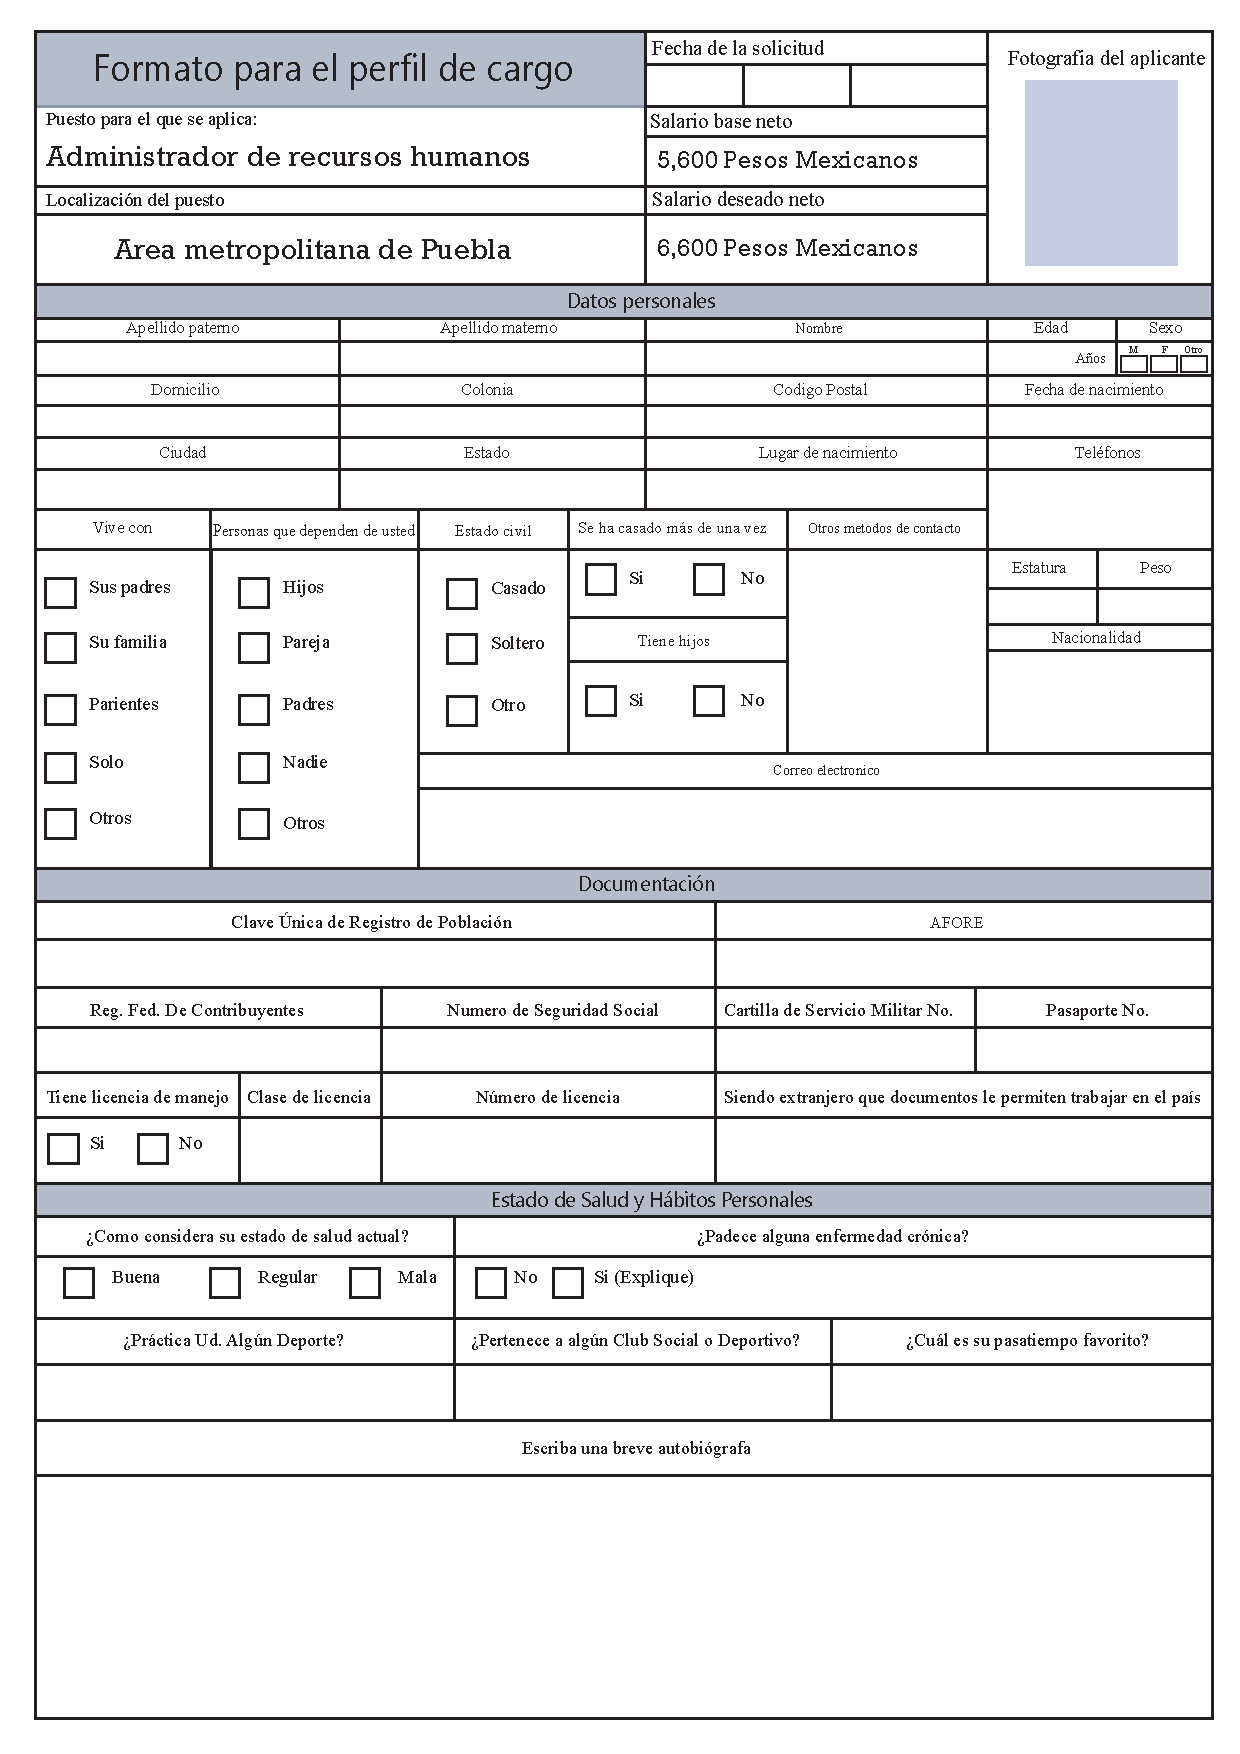
\includepdf[pages=-]{formato_de_empleo (1).pdf}

\newpage

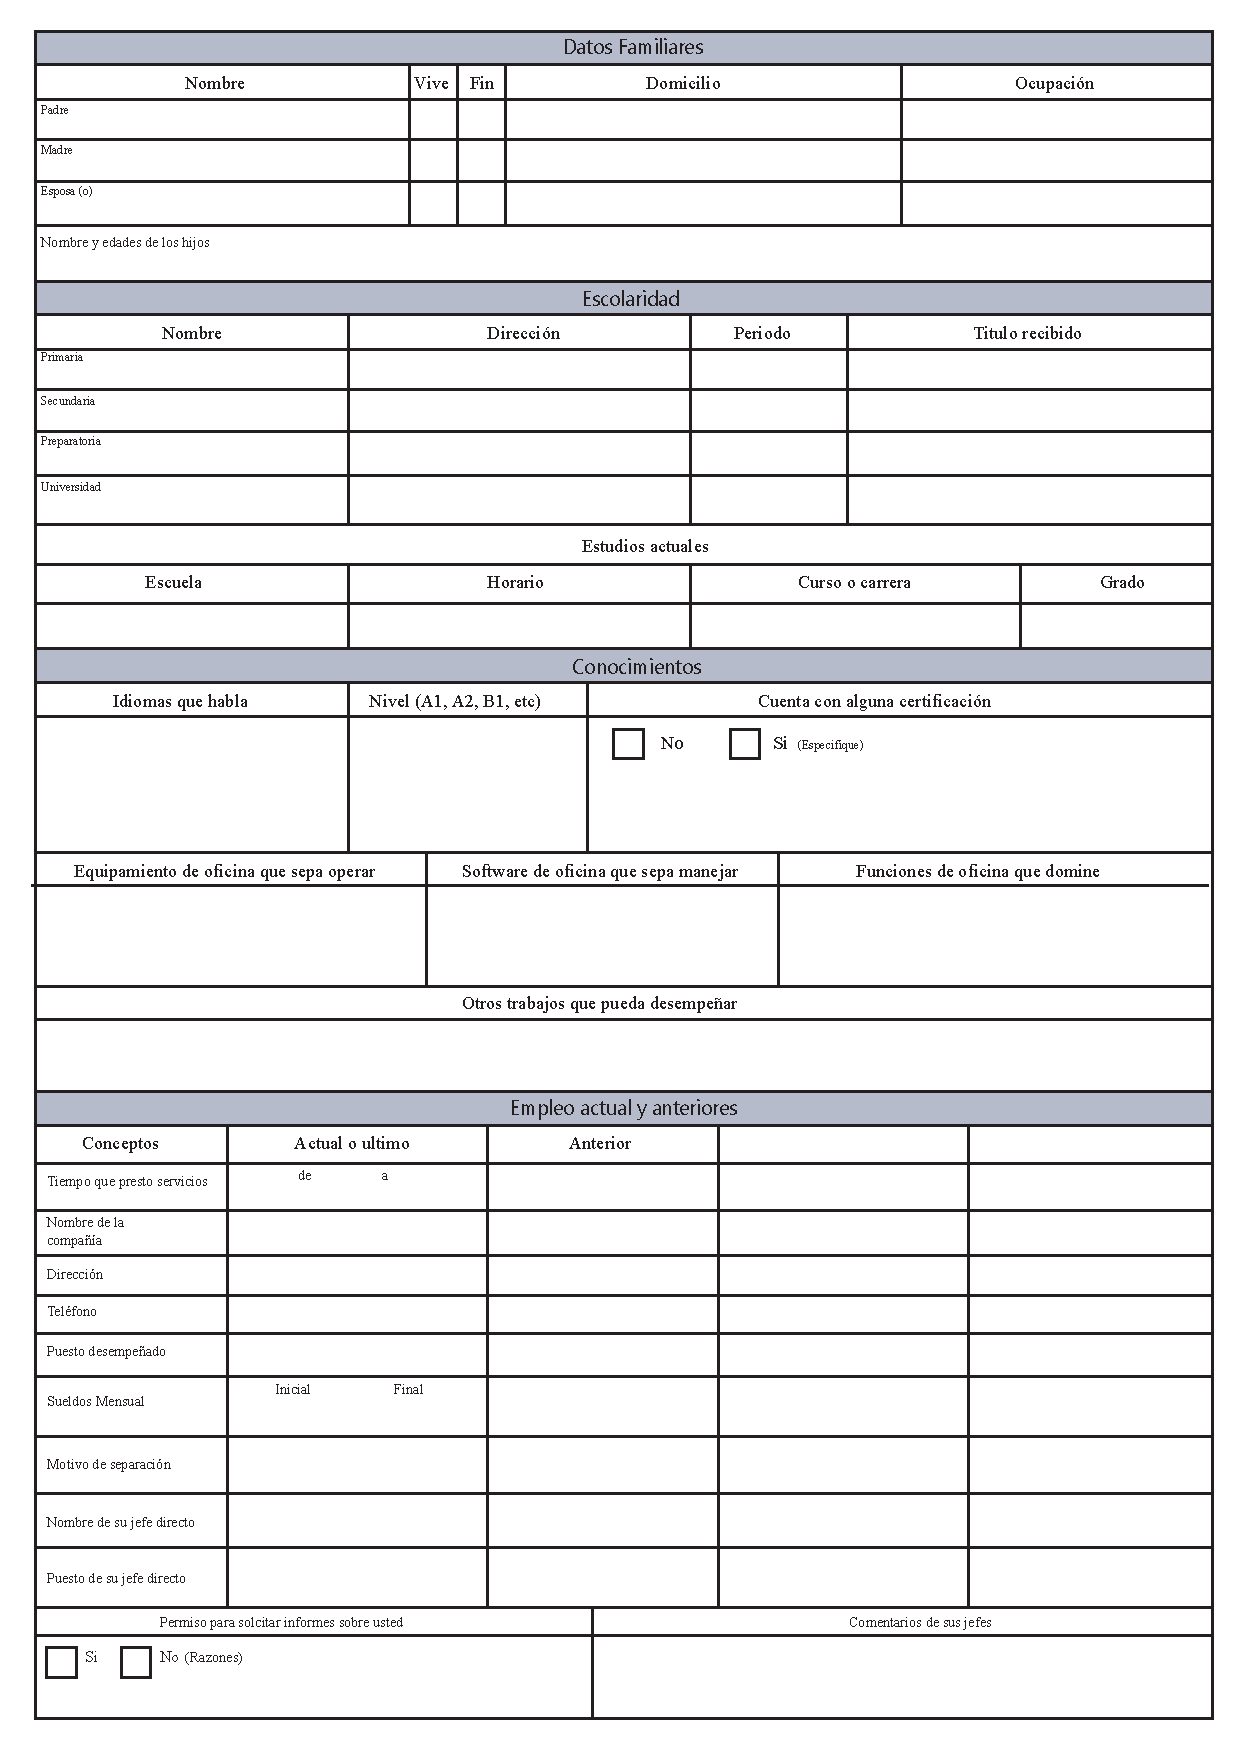
\includepdf[pages=-]{formato_de_empleo-002.pdf}

\newpage 

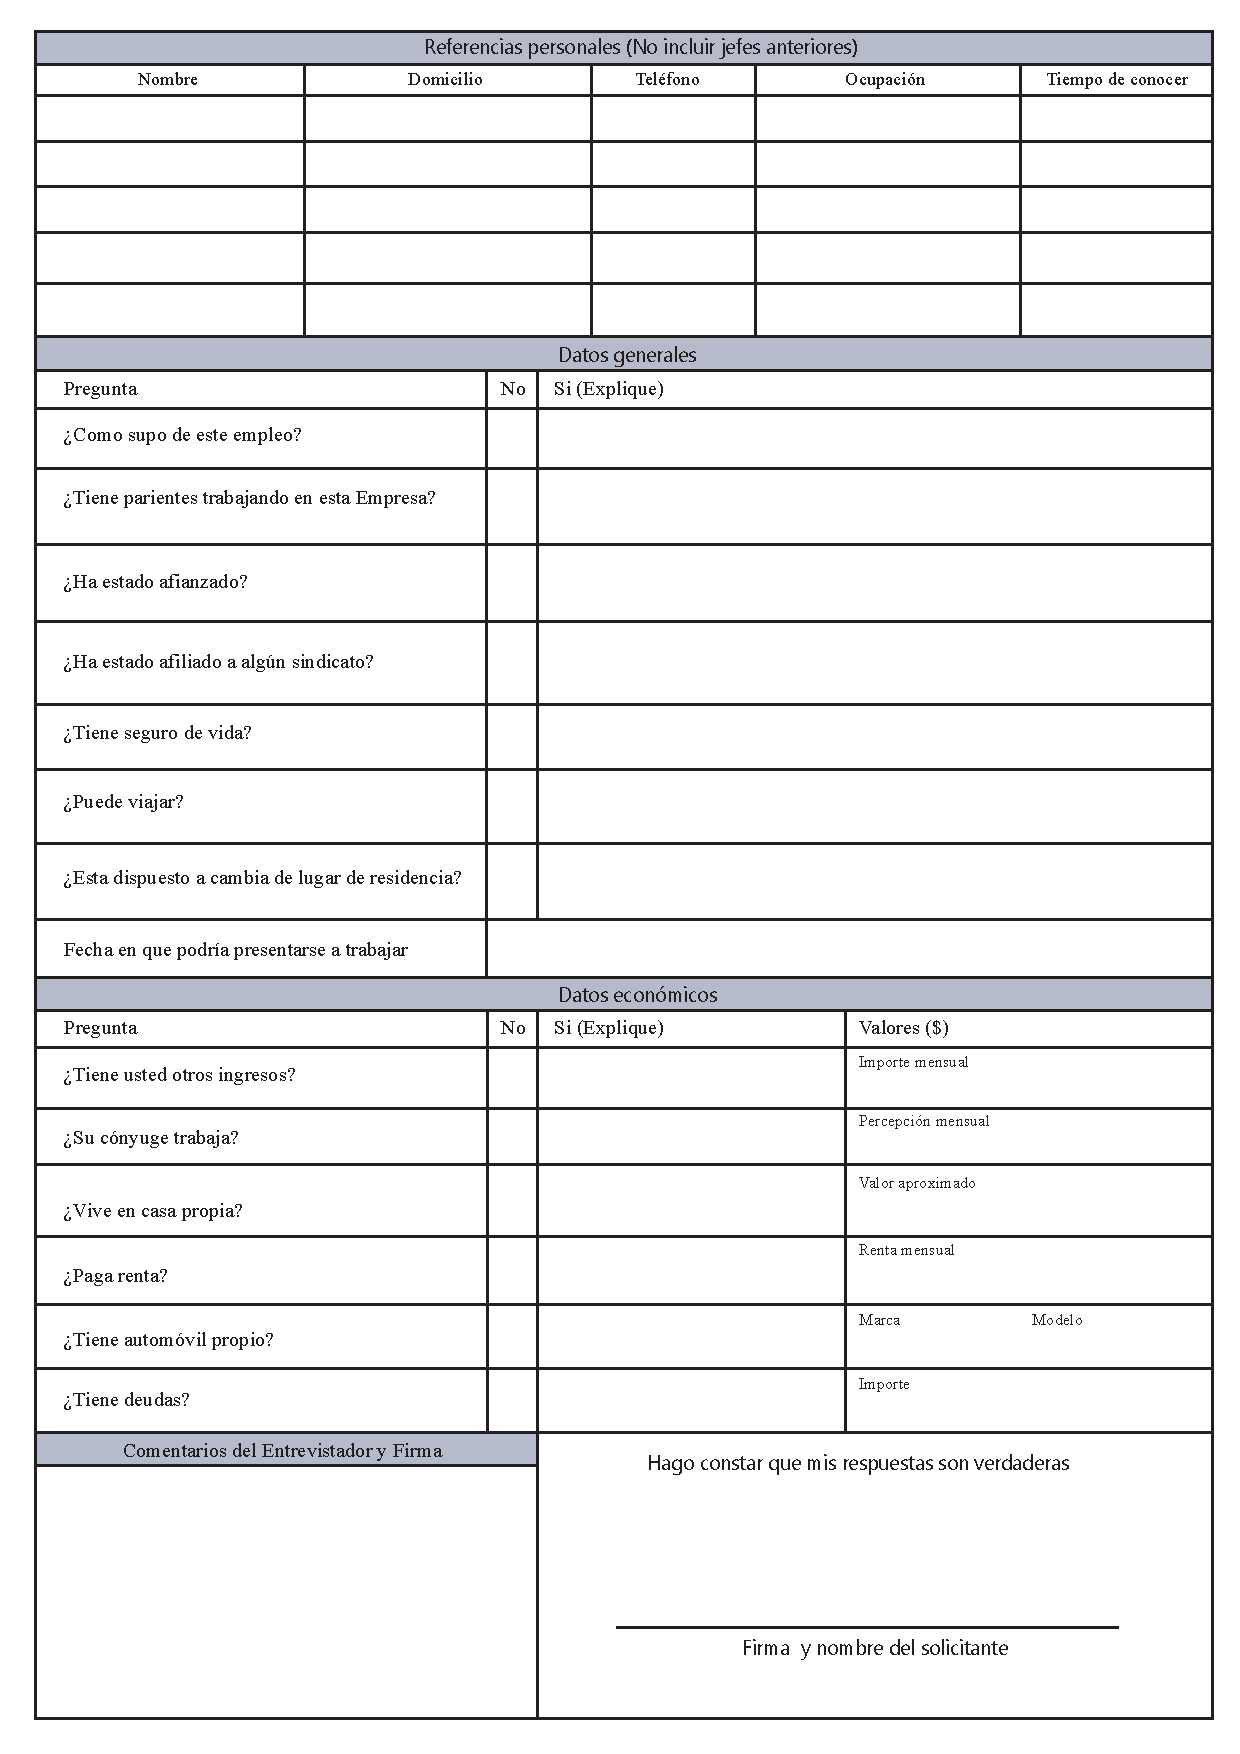
\includepdf[pages=-]{formato_de_empleo-003.pdf}

\subsection{Aviso de privacidad}
En cumplimiento con lo establecido por la Ley Federal de Protección de Datos Personales en Posesión de Particulares, su Reglamento y lineamientos aplicables(en conjunto la "Ley"), en acatamiento al derecho de toda persona a la privacidad y a la autodeterminación informativa, [\textbf{NOMBRE DE EMPRESA, DIRECCIÓN}] 

Para los fines que más adelante se señalan, podrá solicitarle la información que se menciona en el presente Aviso, y en su caso conservar copias de la documentación relativa a la
misma, que será igualmente resguardada con las medidas de seguridad técnicas, administrativas y físicas necesarias para proteger sus datos personales. 

\begin{enumerate}
    \item \textbf{Finalidades de tratamiento de datos personales}
    
    En su relación con los trabajadores se realiza el tratamiento de datos personales de diversa índole que usted libre y voluntariamente le proporcione, para el cumplimiento de las obligaciones a cargo, siendo responsable del uso que se les dé a sus datos personales, única y exclusivamente para los fines que más adelante se mencionan, así como de la protección de los mismos conforme al presente Aviso. 
    
    Conforme a lo anterior, dentro de su objeto social, entre otros, el comercio en general, en su propio nombre o en nombre de terceros incluyendo, pero no limitado a el ensamble, fabricación, producción, elaboración, diseño, compra, venta, importación, exportación, de cualquier tipo de piezas, productos, dispositivos, equipos, partes, autopartes, refacciones, materiales y productos electrónicos, accesorios, y componentes ya sea que estén hechos, de forma enunciativa más no limitativa, de plástico, fibras, resinas, maderas, metales, pieles, o cualquier tipo de material requerido para o en relación con la industria automotriz, la reparación, mantenimiento, instalación y compostura de módulos armados de subconjuntos componentes de automóviles, así como la prestación de servicios especializados o para la ejecución de obras especializadas, bajo cualquier título de apoyo a los negocios que desarrollen las empresas que formen parte del mismo grupo empresarial de la Sociedad ya sea en México o en el extranjero en los términos del artículo 13 de la Ley Federal del Trabajo.

    Conforme a lo anterior, y para efectos del presente Aviso, se hace de su conocimiento que las actividades de recolección, obtención, uso, almacenamiento, acceso y tratamiento de datos personales estarán sujetas a la Ley, su reglamento y disposiciones generales aplicables, siendo
    dichos datos recabados de distintas formas: de manera directa al momento de contratación con la empresa, o de manera indirecta, a través de alguna empresa de reclutamiento, vía telefónica, vía correo electrónico, cuando visita nuestras instalaciones y/o llena algún formato de empleo, datos que ésta utiliza para las siguientes finalidades:

    \begin{itemize}
        \item Para la operación y cumplimiento del objeto social
        \item Llevar a cabo estudios estadísticos relativos al medio ambiente laboral 
        \item Administración de personal, incluyendo expedientes físicos, pago y administración de nímina, prestaciones, pensiones, seguros y demás obligaciones que deriven de la legislación laboral vigente y reglamentos apicables; 
        \item Para asignación de herramientas de trabajo, claves, contraseñas, asegurar obligaciones de confidencialidad, verificar referencias personales y laborales y contactos de emergencia; 
        \item Para cumplimiento de Normas Oficiales Mexicanas vigentes y aplicables a la actividad de la empresa;
        \item Para el ingreso y salida a las instalaciones de la empresa. 
        \item Para el seguimiento a cursos y capacitaciones del persona; 
        \item Para llevar a cabo el proceso reclutamiento, selección y en su caso contratación de personal o bien para ser considerados para ocupar una vacante en alguna de las empresas filiales o pertenecientes a la organización, ya sean nacionales o en el extranjero;
        \item Para la expedición de Pólizas Seguro de Vida y/o Gastos Médicos, si corresponde;
        \item Para documentar la entrada a las instalaciones de FORVIA para efectos de la seguridad del mismo y de las personas que se encuentren en su interior, a través de los sistemas de videovigilancia en las instalaciones de la organización; 
        \item Para la suscripción y cumplimiento de contratos; 
        \item Procesamiento de datos; 
        \item Certificaciones; 
        \item Para transferencias electrónicas interbancarias.
    \end{itemize}
    \item \textbf{Datos personales sujetos a tratamiento }  
    
          Para las finalidades señaladas en el presente aviso de privacidad, recabaremos los siguientes datos personales:

          \begin{itemize}
              \item Personales: nombre, domicilio particular, teléfonos de contacto, correo electrónico personal, fecha de nacimiento, edad, sexo, género, acta de nacimiento (fecha y lugar de nacimiento), nacionalidad, si cuenta o no con doble nacionalidad, datos de identificación, estado civil, firma, RFC, CURP, credencial de elector, entre otros.
              \item Patrimoniales: datos financieros y patrimoniales, bienes, tipo de vivienda, auto propio, información fiscal, historial crediticio, cuentas bancarias, entre otros.
              \item Laborales: número del seguro social (NSS), educación, certificados de estudios, cédula profesional, antecedentes escolares y laborales, resultado de exámenes de aptitudes laborales, psicométricos, coeficiente intelectual, comportamiento laboral y de confiabilidad, entre otros.
          \end{itemize}
        \item \textbf{Obtención de datos personales}
        
        Al realizar actividades de administración de personal (prestaciones laborales, pensiones, seguros y demás prestaciones y/o de obligaciones que deriven de la legislación laboral), de cumplimiento de Normas Mexicanas vigentes, para salvaguardar la seguridad del personal, acceso a las instalaciones de FORVIA, ésta podrá recabar datos personales considerados como sensibles, relacionados con el género, firmas, fotografías, imágenes fijas o en movimiento, afiliaciones sindicales, datos biométricos, geolocalización o posicionamiento global en tiempo real, reconocimiento facial, estado de salud historial clínico, alergias, enfermedades padecidas o que padece, incapacidades, constancias médicas, peso, estatura, presión arterial, temperatura corporal, oxigenación, vacunación, cuestiones de carácter psicológico y/o psiquiátrico, consumo de sustancias tóxicas, datos biométricos, tipo de sangre, procedimientos de emergencia o restricciones a la medicación para lo cual se recabará el consentimiento expreso por escrito del titular para el manejo de dichos datos o la manifestación bajo protesta de decir verdad de quien los proporcione de contar con la autorización y/o representación del titular para facilitarlos. Al proporcionar información a  la organización por cualquier medio, usted confirma que está de acuerdo con los términos de este Aviso de Privacidad, otorgando expresamente su autorización para la recolección, obtención, uso, almacenamiento, acceso y tratamiento de sus datos personales conforme al presente. Si usted no estuviera de acuerdo con cualquier término del Aviso de Privacidad, por favor no proporcione dato personal alguno. Si decide no proporcionar a la organización ciertos datos personales, acepta la posibilidad de no tener acceso a las instalaciones, así como a no tener relación legal con ésta, sin que se genere responsabilidad alguna para ésta última.
        \item \textbf{Transferencia de Datos y tratamiendo por terceros}
        
        para las finalidades previstas en el presente Aviso, podrá:

        \begin{itemize}
            \item Hacer uso de sus datos personales, así como facilitarlos a terceros (personas físicas o
            morales) con quienes tenga contratados servicios y/o departamentos de FORVIA nacionales o internacionales para el procesamiento de datos, para certificaciones, para realizar encuestas y estudios económicos, investigación financiera, auditorías, para que la organización ejerza sus derechos y cumpla con sus obligaciones legales, comprobantes de pago, así como a instituciones bancarias para efectuar transferencias electrónicas.
            \item Transferir sus datos personales para los fines previstos en el presente Aviso, incluidos
            los envíos por correo electrónico, telefonía celular (mensajes SMS, MMS, entre otros) o
            todo medio de comunicación electrónica similar o que pueda llegar a desarrollarse, transferencia que incluye sin limitar, empresas en las que participe o tenga relación de la organización (afiliadas o subsidiarias), incluyendo terceros derivados de una reestructura corporativa, fusión, consolidación, venta, liquidación, o transferencia de activos, así
            como a empresas de consultoría financiera, aseguradoras, empresas que proporcionen
            el servicio de sistema de gestión y almacenamiento de información, para verificarreferencias personales y laborales, auditoría externa, instituciones bancarias,
            aseguradoras, ya sean personas morales o físicas, nacionales o internacionales,
            públicas o privadas, presentes o futuras y en general, para dar cumplimiento a las
            obligaciones que la organización o sus afiliadas y subsidiarias haya contraído con usted, donde
            sólo se proporcionarán los datos personales que sean indispensables para la actividad
            o servicio específico que dichas terceras personas realizarán.
            \item Transferir sus datos personales a cualquier otra sucursal u oficina al interior del país o
            en el extranjero, y/o a cualquier servidor de respaldo de información en México o en el
            extranjero.
            
        \end{itemize}
        
        
\end{enumerate}


\section{\textcolor[rgb]{0.4,0.4,0.9}{Instrumentos de evaluación a candidatos}} 
\subsection{Entrevista colectiva}
Antes de mostrar nuestro modelo y étapas de la entrevista \textit{(Anexo \ref{fig:6})}, se revisará brevemente las definiciones de otros autores: 
\begin{itemize}
    \item 'Una entrevista es una conversación a propósito. Es un proceso interactivo que involucra muchos aspectos de la comunicación que el simple hablar o escuchar, como ademanes, posturas, expresiones faciales y otros comportamientos comunicativos' (Morgan y Cogger, 1975)
    \item 'En una organización es, principalmente, una situación vocal en un grupo de dos, más o menos voluntariamente intregado sobre una base de desarrollo progresivo de experto-cliente, con el propósito de elucidar pautas características de vida del sujeto entrevistado, y qué pautas y normas experimenta como particularmente productoras de dificultades o le parecen valiosas en la revelación de las cuales espera obtener algún beneficio' (Sullivan, 1977) \textit{(Anexo \ref{fig:7})}
\end{itemize}
\subsubsection{Etapas de entrevista}
\begin{enumerate}
    \item \textbf{Apertura} :  Aquí ambos tienen la primera impresión o impacto ya que se conocen por primera vez. 
    \item \textbf{Rapport} : Pequeña charla casual por cortesía entre entrevistado-entrevistador, para disminuir la ansiedad del solicitante y poder crear un clima de confianza, espontaneidad. Esto provoca que el entrevistado se comporte de modo natural de acuerdo con las circustancias del momento. También es importante aclarar que la \textbf{información se tratará de manera confidencial, preservando la privacidad del entrevistado}(Aviso de privacidad, pg. 5) %%%%%%%%%%%%%%%%%%%%%%%%%%%%%%%%%%%%%%%%%%%%%%%%%%%%%%%%%%%%%%%%%%%%%%%%
    
    En este momento podemos preguntar cosas como: \textit{"¿No tuvo problemas para estacionarse?", "¿Vino desde muy lejos?", "¿Hacía frío afuera?", "Que bien cortado está su traje".} 
    \item \textbf{Approach} : Poner a la persona en condiciones antes de empezar con la entrevista, desde el punto de vista sociopsicológico se le denomina la distancia social o distancia psicológica que existe entre dos personas. Se presentarán condiciones los cuales el entrevistador esté de acuerdo, si hablar de "tuteo" o de "usted" \textit{-por ejemplo-}. 
    \item \textbf{Desarrollo} : Acá obtenemos la mayor cantidad de información, esto es posible porque se ha establecido un buen \textit{rappot} y existe un clima de confianza, donde el entrevistado presenta una mayor solidez y se obtiene información cada vez más significativa.
    
    Preguntas como \textit{"¿Dónde vive usted?", "¿Dónde estudió la primaria?", "¿Por qué quieres trabajar aquí?", "¿Tienes trabajos anteriores? Si es así, ¿Cómo fue el ambiente?", "¿Cuáles son tus pasatiempos?", "¿En qué te consideras bueno?", "¿Cuál consideras que es tu mayor debilidad?", "¿Cuáles han sido tus experiencias laborales previas relacionadas con la gestión de recursos humanos?", "Cuentame de tu experiencia laboral..."}

    Entre otras cosas, también se preguntan sus habilidades técnicas: \textit{"¿Podrías resumir tu conocimiento en leyes laborales?", "Comentame tu experiencia con diferentes herramientas o sistemas con los que has trabajado para un análisis"}

    El esquema se centraría de igual forma sobre preguntas situacionales, conductuales o conocimiento de empresa e industria: \textit{"¿Cómo manejarías una situación de conflicto entre empleados?", "¿Cómo implementarías una nueva política de recursos humanos?","¿En qué proyectos o iniciativas lideraste?", "¿Qué resultado has obtenido dentro de tus roles anteriores?", "¿Qué entiendes por desafíos dentro de la industria?"}
    \item \textbf{Cima} : Se centrará en obtener información cualitativa más significativa, realizando preguntas abiertas (algunos autores denominan preguntas exploratorias o de sondeo) para abordar áreas que no hayan quedado claras, dando pauta a cosas como: \textit{"Hábleme más de sus estudios" o "Cuénteme más sobre su familia"}
    \item \textbf{Cierre} : De cinco a tres minutos antes de terminar la entrevista se anunciará que se acerca el final con transacciones como la siguiente: \textit{"He disfrutado haber conversado con usted" o "Le agradezco haber compartido esta información conmigo"}
\end{enumerate}

\section{\textcolor[rgb]{0.4,0.4,0.9}{Prototipo de entrevista a candidato para \textit{Administrador de Recursos Humanos}}}
Sabiendo el proceso de entrevista colectiva, nos hemos dado el trabajo de presentar nuestra propia entrevista en base a un \textit{Administrador de Recursos Humanos}.
\vspace{0.3cm}\\ 
Es necesario saber que a continuación se muestra nuestro trabajo con un \textbf{profundo análisis} en base a nuestro críterio, se puede tomar como una especie de "miniguía" para el propio entrevistador y, en base a esto, pueda hacer más preguntas para indagar; tal es esto porque tomamos en cuenta factores que puedan perjudicar la entrevista, por ejemplo, que no todas las personas se van a comportar igual dependiendo de factores (modales de el entrevistado), incluso el estado de ánimo que tenga o ciertas dificultades con el día o la hora de la entrevista.
\vspace{0.3cm}\\ 
Estos factores hacen que debamos tener en cuenta que un método rígido de contratación que nos daría los mejores resultados para conseguir al personal con mayor capacidad posible ya que no podemos medir a todas las personas con la misma regla porque no todas las personas son iguales. 
\vspace{0.3cm}\\ 
Para empezar lo obvio, ¿cómo fue el camino? Si encontró el lugar rápido o incluso puede ser una pregunta de algo que paso en días relevantes. 

De ahí se iría algo mas como notar un detalle de la ropa para ver un poco más de la personalidad o algo diferente que pueda decir un poco más de como es, y de hecho, primero que nada, hay que preguntar cosas un poco básicas como de donde viene la persona y su familia, como creció y para que nos den un contexto explícito: 
\begin{center}
    ¿De dónde eres?

    ¿Dónde creciste?

    ¿Cómo fueron tus padres?

    ¿Tienes hermanos? ¿Cómo son?
\end{center}
Ya después de un par de preguntas así podemos empezar con cosas como
\begin{center}
    ¿Dónde fuiste a la primaria?  Secundaria, bachillerato, universidad, etc 
\end{center}
Si fue a una escuela o a varias privadas, referencias de un maestro o algo que sea relevante, una certificación de un curso o un diploma que tenga.

Después de eso ya podemos empezar con algo más personal, tal como si tiene hijos, tiene más de un matrimonio o tiene que pagar una pensión. También así podríamos saber si es una persona medio difícil de trabajar dependiendo de la información que nos diga, un ejemplo de como podríamos saber esto es que si se divorció por culpa suya, no se puede ver como alguien muy confiable.
\begin{center}
    ¿Cómo son tus hijos?

    ¿Pasas mucho tiempo con ellos?

    ¿Tienes alguna pareja?

    ¿Vives con tu pareja?
\end{center}
Luego se preguntan cosas un poco más sencillas como por ejemplo, si hace algún deporte --para indagar un poco más en cómo es su salud-- o si mantiene un estilo de vida sano que, realmente, viéndolo desde contratar una persona enfermiza que tal vez falte diario o que tenga situaciones similares, no es la mejor opción.

Las preguntas que hacemos deben de tener como objetivo el obtener más información de parte del entrevistado llevando a una conversación orgánica en la que el entrevistador pueda tener una mirada más cercana a el verdadero comportamiento de la persona y, así evitar situaciones que harían más difícil el proceso de contratación, sin embargo, esto también vendría con un par de desventajas a la productividad ya que el entrevistador tendría que estar capacitado para notar detalles en el comportamiento y en las actitudes del aspirante, por lo que no podría ser cualquier tipo de entrevistador. 
\vspace{0.3cm}\\ 
Dentro del contexto de una empresa de mayor magnitud como lo es Faurecia, tendría todo el sentido del mundo que un entrevistador bien capacitado, con los conocimientos suficientes y con la experiencia para entender a las personas que solicitan el empleo, sean las indicadas para este tipo de tabajo. Ahora bien, sabiendo que el entrevistado esperará causar la mejor impresión, es importante considerar que siempre existirá la probabilidad de que tal vez mienta en datos que no podemos confirmar fácilmente (como relaciones personales, hobbies o gustos)  con la intención de contribuir a su contratación lo cual el encargado de las preguntas deberá estar al pendiente de señales como esas, patrones de comportamiento como esos pueden ser medidos con un entrevistador ilustrado y experimentado con las personas. 
\vspace{0.3cm}\\ 
Hemos propuesto tener un par de preguntas de control para utilizar como ayuda para que el entrevistador pueda corroborar cualquier sospecha de que una persona puede estar mintiendo --como por ejemplo el repetir preguntas con diferentes palabras--. Todo esto sería de gran ayuda ya que daría una oportunidad de confirmar o desmentir sospechas que ayudaría a una mayor confiabilidad en el momento del contrato de personal.
\newpage
\subsection{Test psicométrico}

Este consistira en probar de una forma mas profunda a los candidatos que quieran ir al puesto de Administrador de Recursos Humanos. Estas preguntas van a probar tanto la percepcion hacia si mismo y los demas como los pensamientos que se tiene hacia el entorno del mismo. 
\vspace{0.3cm}\\ 
\noindent Dentro de este test se le va a preguntar al aplicante preguntas como por ejemplo:

\begin{itemize}
    \item Termina esta oración: Me considero una persona \_\_\_\_\_\_\_\_\_
    \item Sea $8x + 3 = 25$. Encuentre el valor de x.  
    \item ¿Es capaz de organizar de forma efectiva un trabajo colectivo?
    \item ¿Te gusta ir a reuniones sociales?
    \item Soy una persona incompetente. ¿Está de acuerdo con esta oración?
\end{itemize}

Algunos otros tipos de test que se incluyen son: 
\begin{itemize}
    \item Test de Raven: que determina concentración, lógica y observación.
    \item Test de Terman Merril: mide el coeficiente intelectual, y su aplicación más habitual es en posiciones administrativas, supervisores, coordinadores y similares.
    \item Test de Cleaver: describe la reacción ante una situación estresante y el desarrolla del trabajo en esa condición. 
    \item Test de Moss: se clasifica dentro de la categoría de pruebas psicométricas que miden la adaptabilidad social de la persona con el objetivo de conocer y predecir su comportamiento.
    \item Test 16PF: identifica 16 rasgos que tenemos en diferentes proporciones. Este test, de los más usados, tiene 170 preguntas, determina cómo respondemos a situaciones laborales, y es conveniente para altos y medios mandos.
    \item OPQ32: muestra cómo los rasgos influyen en el desempeño laboral, tiene 104 preguntas, mide 32 características, y se basa en escoger las opciones más y menos parecidas a la personalidad del postulante
\end{itemize}

De acuerdo a las respuestas que conteste el aplicante tendremos expectativas acerca del mismo en el ámbito socio-laboral; nos dará una idea de cómo interactuará con los trabajadores y en las decisiones que se deban de tomar, las funciones que este vaya a ejecutar en su puesto, el control y la gestión que manejará en los recursos humanos, entre otras acciones que este vaya a tomar. Esto lo tomaremos en cuenta junto con otras evaluaciones para determinar si alguno de los aplicantes es admitido a la organización para ese puesto.

\begin{center}
    \textbf{Citamos un software con el nombre de 'bizneo' que realiza la selección por competencias automáticamente a los mejores candidatos en función de cómo encajan con la descripción de la vacante. (Anexo \ref{fig:7}) }
    \vspace{0.3cm}\\ 
    $https://www.bizneo.com/reclutamiento-seleccion-ats/?utm_content=post-imagen$

\end{center}
\newpage
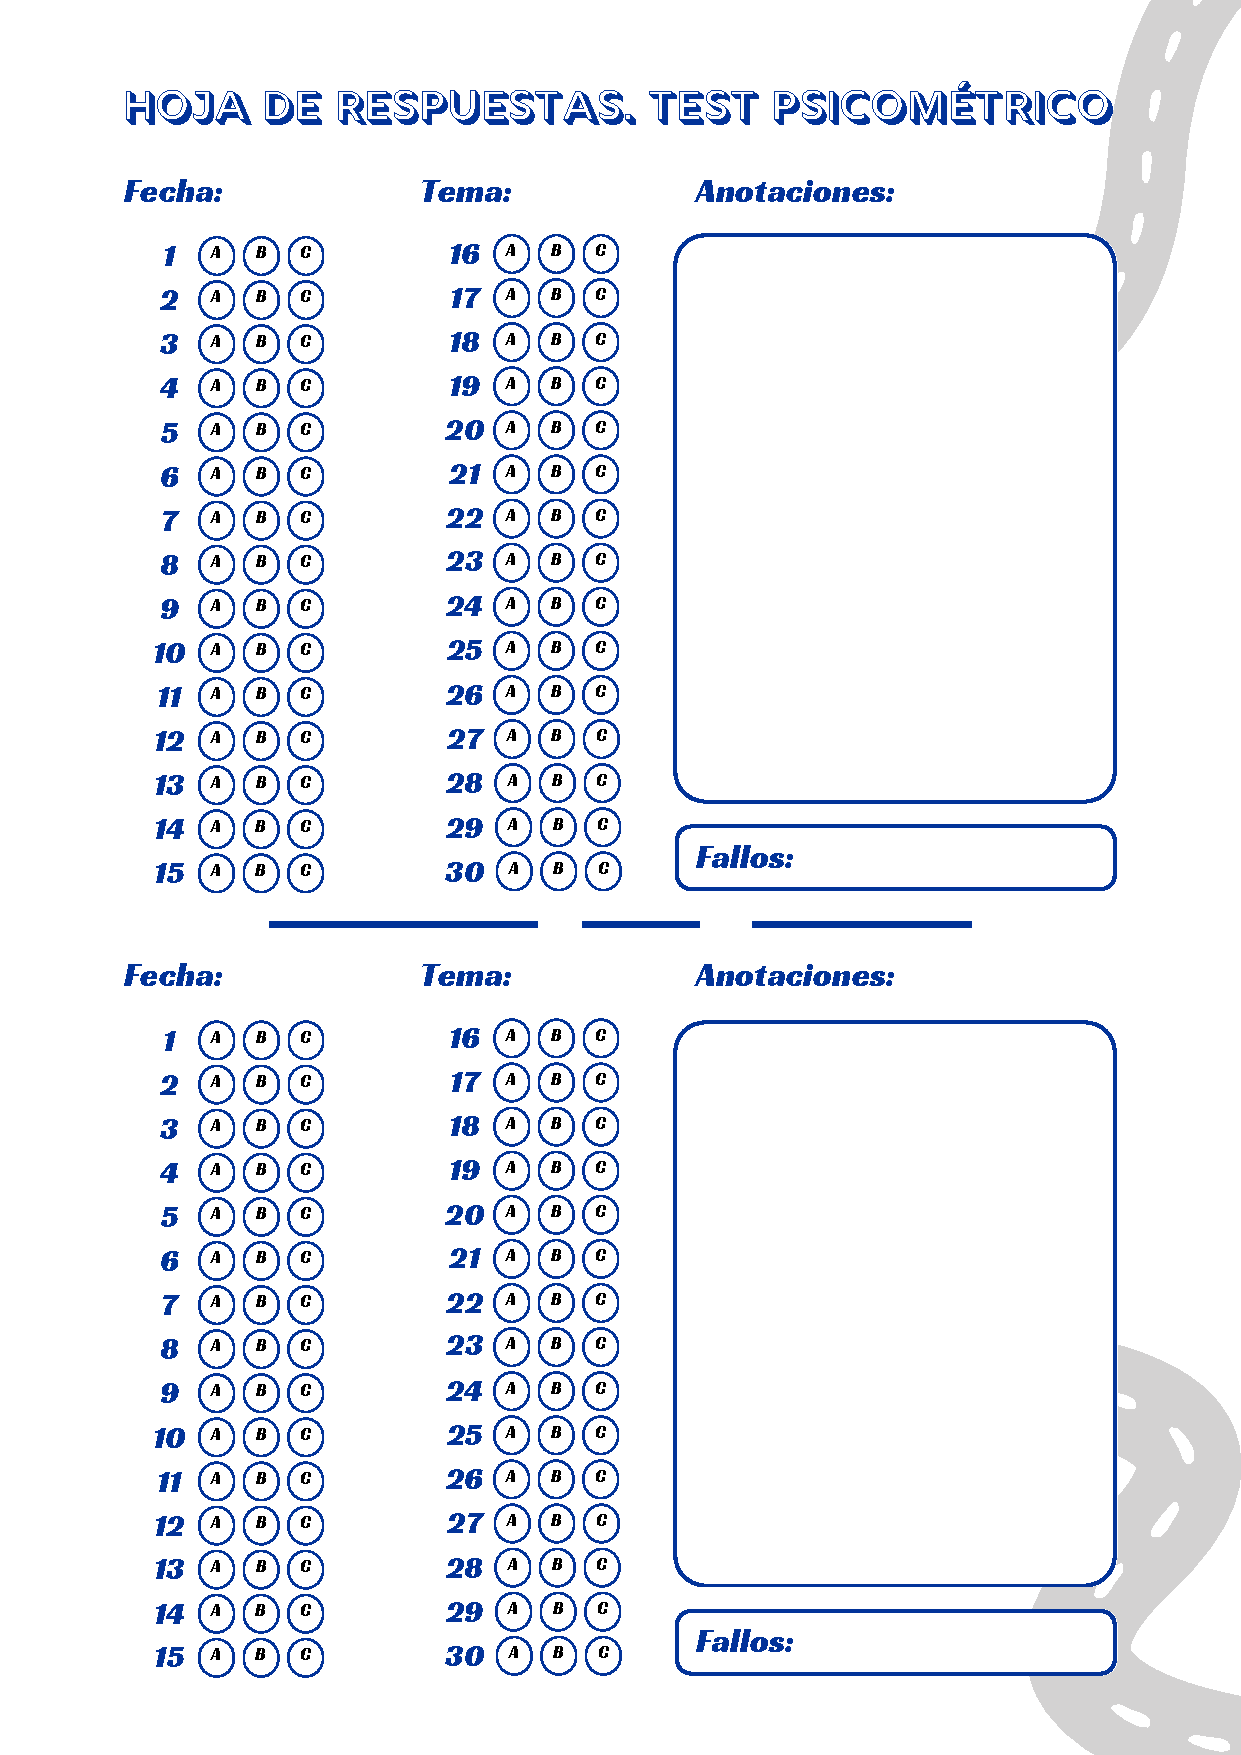
\includepdf[pages=-]{test.pdf}
\subsection{Prueba técnica de habilidades}

Es importante incluir ejercicios diseñados para evaluar las habilidades del candidato, a continuación se presenta el proceso para el cargo el cual se evaluará las competencias técnicas y de conocimiento.
\begin{enumerate}
    \item \textbf{PRUEBA TEÓRICA DE CONOCIMIENTOS ADMINISTRATIVOS}: 15 preguntas de selección múltiple con una duración de 50 minutos
    \item \textbf{PRUEBA DE VALOR AGREGADO CULTURAL:} evalúa cómo los valores y comportamientos de un candidato se alinean con los valores de la organización y los comportamientos que harían que el postulante ideal tuviera excelentes resultados en un puesto específico. Tiene una duración de 10 minutos. 
    \item \textbf{PRUEBA DE PENSAMIENTO CRÍTICO (habilidad cognitiva):} evalúa las habilidades de pensamiento crítico de los candidatos a través de problemas de razonamiento inductivo y deductivo. Este test de habilidades pre-empleo le ayudará a identificar a los candidatos que pueden evaluar la información y hacer juicios sólidos utilizando habilidades analíticas. Tiene un tiempo de 10 minutos.
    \begin{itemize}
        \item Resolución de silogismos (razonamiento deductivo)
        \item Interpretación de secuencias y disposiciones
        \item Comprensión de las relaciones de causa y efecto
        \item Interpretación de secuencias y disposiciones
    \end{itemize}
    \item \textbf{PRUEBA DE TI:} evalúa las habilidades técnicas de los candidatos en el uso de la plataforma Microsoft 365 (Exchange Online, Azure Active Directory, SharePoint y Microsoft Teams) y su capacidad para evaluar, diseñar, implementar y administrar servicios de Microsoft 365. Tiempo de 10 minutos.
    \item \textbf{PRUEBA DE MANEJO DE DATOS:} se evalúa la capacidad de cada candidato o candidata para trabajar con datos, incluyendo su manejo correcto y la realización de análisis básicos de datos.  Tiene duración de 10 minutos
    \begin{itemize}
        \item Compresión de los conceptos de manejo de datos 
        \item Trabajo con gráficos y diagramas 
        \item Realización de análisis e interpretación de datos básicos
    \end{itemize}
    \item \textbf{PRUEBA DE INGLÉS B1:} evalúa el dominio del inglés del candidato en el nivel B1 del Marco Común Europeo de Referencia (MCER) para las lenguas. Duración de 30 min.
    \begin{itemize}
        \item Gramática y vocabulario básicos
        \item Composición de oraciones
        \item Comprensión auditiva
        \item Comprensión de lectura
    \end{itemize}
\end{enumerate}

\section{\textcolor[rgb]{0.4,0.4,0.9}{Conclusiones individuales}}

\noindent (Martínez Schleske Alan)

El objetivo de un Administrador de Recursos Humanos es de gestionar, manejar y controlar aquellos recursos que la organización requiera para la elaboración de un producto, sea para el mercado o para uso laboral\dots

Para evaluar a aquellos que quieran aplicar al puesto necesitamos un conjunto de evaluaciones de contratación para llevar a cabo esa decisión. Entre esas evaluaciones se aplican tests psicométricos, los cuales ponen a prueba el pensamiento tanto crítico como psicológico del candidato; entrevistas para conocer bien al mismo para observar la interacción que tendrá con los trabajadores; y pruebas técnicas en las que el aplicante pone a prueba sus conocimientos previos para su aplicación en el puesto. 
\vspace{0.3cm}\\
(Lara Xocuis Martha Denisse)

Un administrador es una parte muy importante y fundamental dentro del ambiente empresarial, este mismo no solo se encarga de la dirección y flujo económico de dicha empresa, también es una imagen a seguir dentro de dicha empresa tanto para los empleados y organizaciones externas que estén vinculadas.

Dentro de la dirección de una organización, objetivos y funciones, es donde se encuentra dicho Administrador, indagar profundamente en otras instituciones como Faurecia nos dan un vistazo más amplio sobre las habilidades sociales y gestiones en cuanto a los puestos de trabajo. 
\vspace{0.3cm}\\ 
(López Castillo Haziel)

El rol del administrador es muy importante ya que se encargará de mantener el orden y la productividad de la empresa en los sectores bajo su encargo. En la búsqueda de empleados competentes se necesitan varias estrategias y muchas herramientas que facilites el trabajo dándonos un mejor entendimiento y tomar mejores decisiones que ayuden a la empresa, estas herramientas deberán ser desarrolladas por diferentes personas en diferentes campos de trabajo como la psicología o administración ya que se necesita un amplio rango de habilidades para hacer un trabajo más efectivo.

\newpage
\section{\textcolor[rgb]{0.4,0.4,0.9}{Aprendizaje individual}}

\noindent (Martínez Schleske Alan)

Tengo la idea de cómo gestionaré ciertos factores para organizar una empresa de manera efectiva (gestionar los recursos con las que dispone mi empresa), qué debo de tener en cuenta en orden de jugar el papel de un administrador (los requerimientos necesarios para trabajar en ese puesto), cuándo y cómo tomaré decisiones dependiendo de la situación con la que se enfrente mi empresa (si es una situación muy impactadora como un cambio en las normas laborales, planear una estrategia para mantener o mejorar la condicion tanto de los trabajadores como del estado de la empresa), y cómo evaluaré a alguien que quiera entrar dentro de ese puesto, utilizando los instrumentos de evaluación que se especificaron.
\vspace{0.3cm}\\
(Lara Xocuis Martha Denisse)

Buscar información de forma más minuciosa y profunda --considero-- que no solo fue la parte más importante de todo lo que aprendí en este trabajo, fue interesante y enriquecedor adentrarme dentro de la gestión organizacional porque realmente no es solo el tener una meta y conseguir un objetivo, es tener también una actitud, planeación, habilidad y acción al momento de hacer las cosas. También dentro de una evaluación y cosas necesarias para seguir con la competitividad es otra parte muy fundamental que aprendí a lo largo de este proyecto.
\vspace{0.3cm}\\
(López Castillo Haziel)

Ahora entiendo de mejor manera el proceso que se lleva en una empresa y como funciona en el mundo real, todo lo que implica el análisis de los datos y de las habilidades necesarias de las que se debe tener en cuenta para aumentar las probabilidades de conseguir el mejor empleado posible junto con las interesantes estrategias que se necesitan para asegurar un mejor proceso de administración. También he aprendido que es un trabajo de el que se necesita un conjunto de personas diferentes con habilidades distintas para logar crear y diseñar las herramientas necesarias para este tipo de aplicaciones al mundo laboral.



\newpage
\section{\textcolor[rgb]{0.4,0.4,0.9}{Bibliografía}}
\textit{Ouest-France. (2022b, February 8). Faurecia devient Forvia : ce qu'il faut savoir sur ce nouveau géant de l'industrie automobile. https://www.ouest-france.fr/}
\vspace{0.3cm}\\ 
\textit{Europa Press. (n.d.). Faurecia vende parte de su negocio de vehículos comerciales en Europa y EEUU a Cummins por 142 millones. europapress.es. https://www.europapress.es/motor/sector-00644/noticia-faurecia-vende-parte-negocio-vehiculos-comerciales-europa-eeuu-cummins-142-millones-20230525181132.html}
\vspace{0.3cm}\\ 
\textit{History of Faurecia S.A. – FundingUniverse. (n.d.). http://www.fundinguniverse.com/company-histories/faurecia-s-a-history/}
\vspace{0.3cm}\\ 
\textit{Faurecia S.A. -- Company History. (n.d.). https://www.company-histories.com/Faurecia-SA-Company-History.html}
\vspace{0.3cm}\\ 
\textit{Our companies | FORVIA, inspiring mobility. (n.d.). FORVIA, Inspiring Mobility. https://www.forvia.com/who-we-are/our-companies}
\vspace{0.3cm}\\ 
\textit{Faurecia SA Company Profile - Faurecia SA Overview. (n.d.). GlobalData. https://www.globaldata.com/company-profile/faurecia-sa/}
\vspace{0.3cm}\\ 
\textit{Edward Hoffman. (n.d.). Tests Psicológicos.}
\vspace{0.3cm}\\ 
\textit{¿Qué hace un administrador de Recursos Humanos? (2022, January 19). https://www.crehana.com. https://www.crehana.com/blog/upskilling-reskilling/administrador-de-recursos-humanos/}
\vspace{0.3cm}\\ 
\textit{De Ceupe, B. (2022). ¿Qué estudiar para trabajar en el área de Recursos Humanos? Ceupe. https://www.ceupe.com/blog/}
\vspace{0.3cm}\\ 
\textit{Perfil de Gerente de Recursos Humanos. (n.d.). Hireline. https://hireline.io/mx}
\vspace{0.3cm}\\ 
\textit{Perfil del puesto de administrador de recursos humanos - Primera Base. (2021, July 21). Primera Base. https://primerabase.com/perfil-de-puesto-de-administrador-de-recursos-humanos/}
\vspace{0.3cm}\\ 
\textit{Salario para Administrador De Recursos Humanos en México - Salario Medio. (n.d.). Talent.com. https://mx.talent.com/salary?job=administrador+de+recursos+humanos}
\vspace{0.3cm}\\ 
\textit{Andrés, Á. (2022). 8 pruebas psicométricas clave en reclutamiento y selección. Blog De Recursos Humanos De Bizneo HR: Práctico Y Actual. https://www.bizneo.com/blog/ejemplos-pruebas-psicometricas-seleccion/}
\vspace{0.3cm}\\ 
\textit{La entrevista en las organizaciones. 3a edición. Ángel Jaime Grados Espinoza. Elda Luisa Sánchez Fernández}
\vspace{0.3cm}\\ 
\textit{Módulo Didáctico: Pruebas psicométricas. Hernández Calle; Jonathan Andrés}
\vspace{0.3cm}\\ 
\textit{El Administrador: Concepto, Perfil y Funciones. UNAM}
\vspace{0.3cm}\\ 
\textit{Aviso de privacidad. FAURECIA SISTEMAS AUTOMOTRICES DE MÉXICO, S.A. de C.V.
SERVICIOS CORPORATIVOS DE PERSONAL ESPECIALIZADO, S.A. de C.V.}

\section{\textcolor[rgb]{0.4,0.4,0.9}{Anexos}}

\begin{figure}[H]
    \centering
    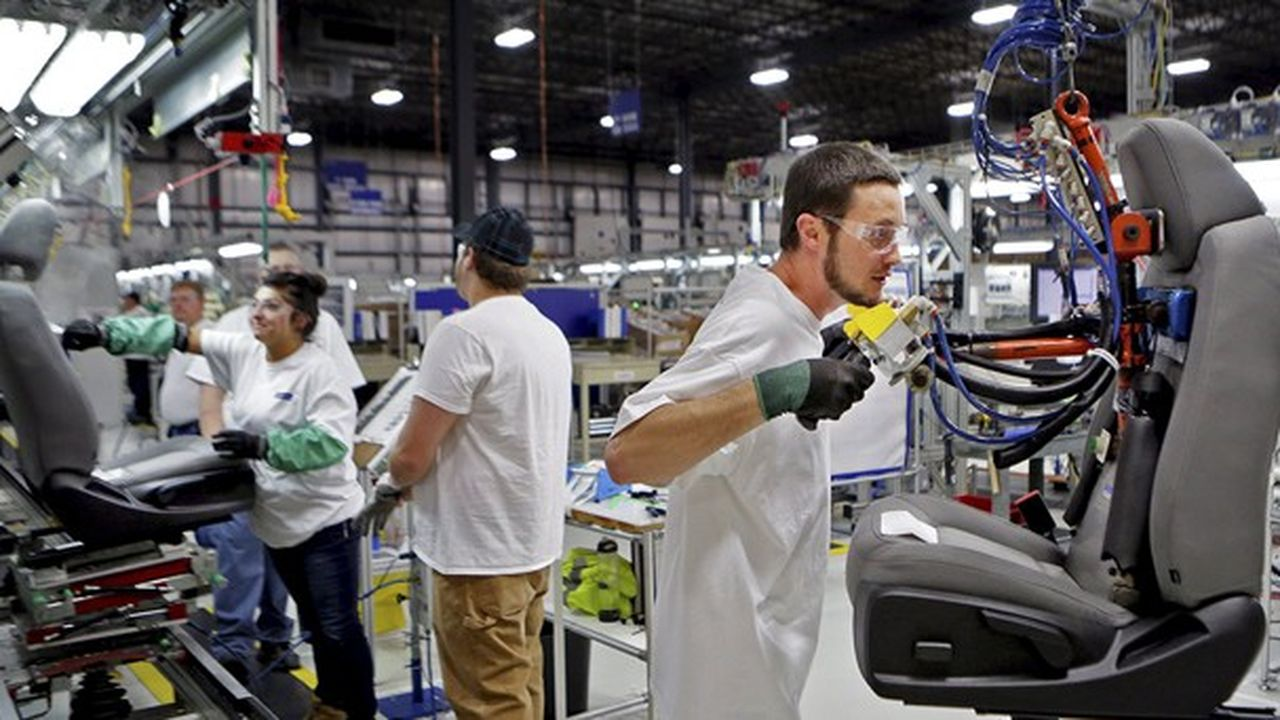
\includegraphics[width=0.4\textwidth]{images/faurecia.jpg}
    \caption{Empresa de Faurecia}
    \label{fig: 1 }
    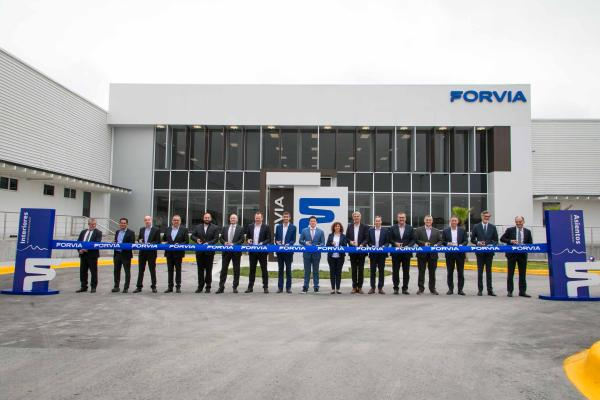
\includegraphics[width=0.4\textwidth]{images/faureciamexico.jpg}
    \caption{Faurecia México}
    \label{fig: 2}
    %%%%subfiguras
    \begin{subfigure}{0.3\textwidth}
        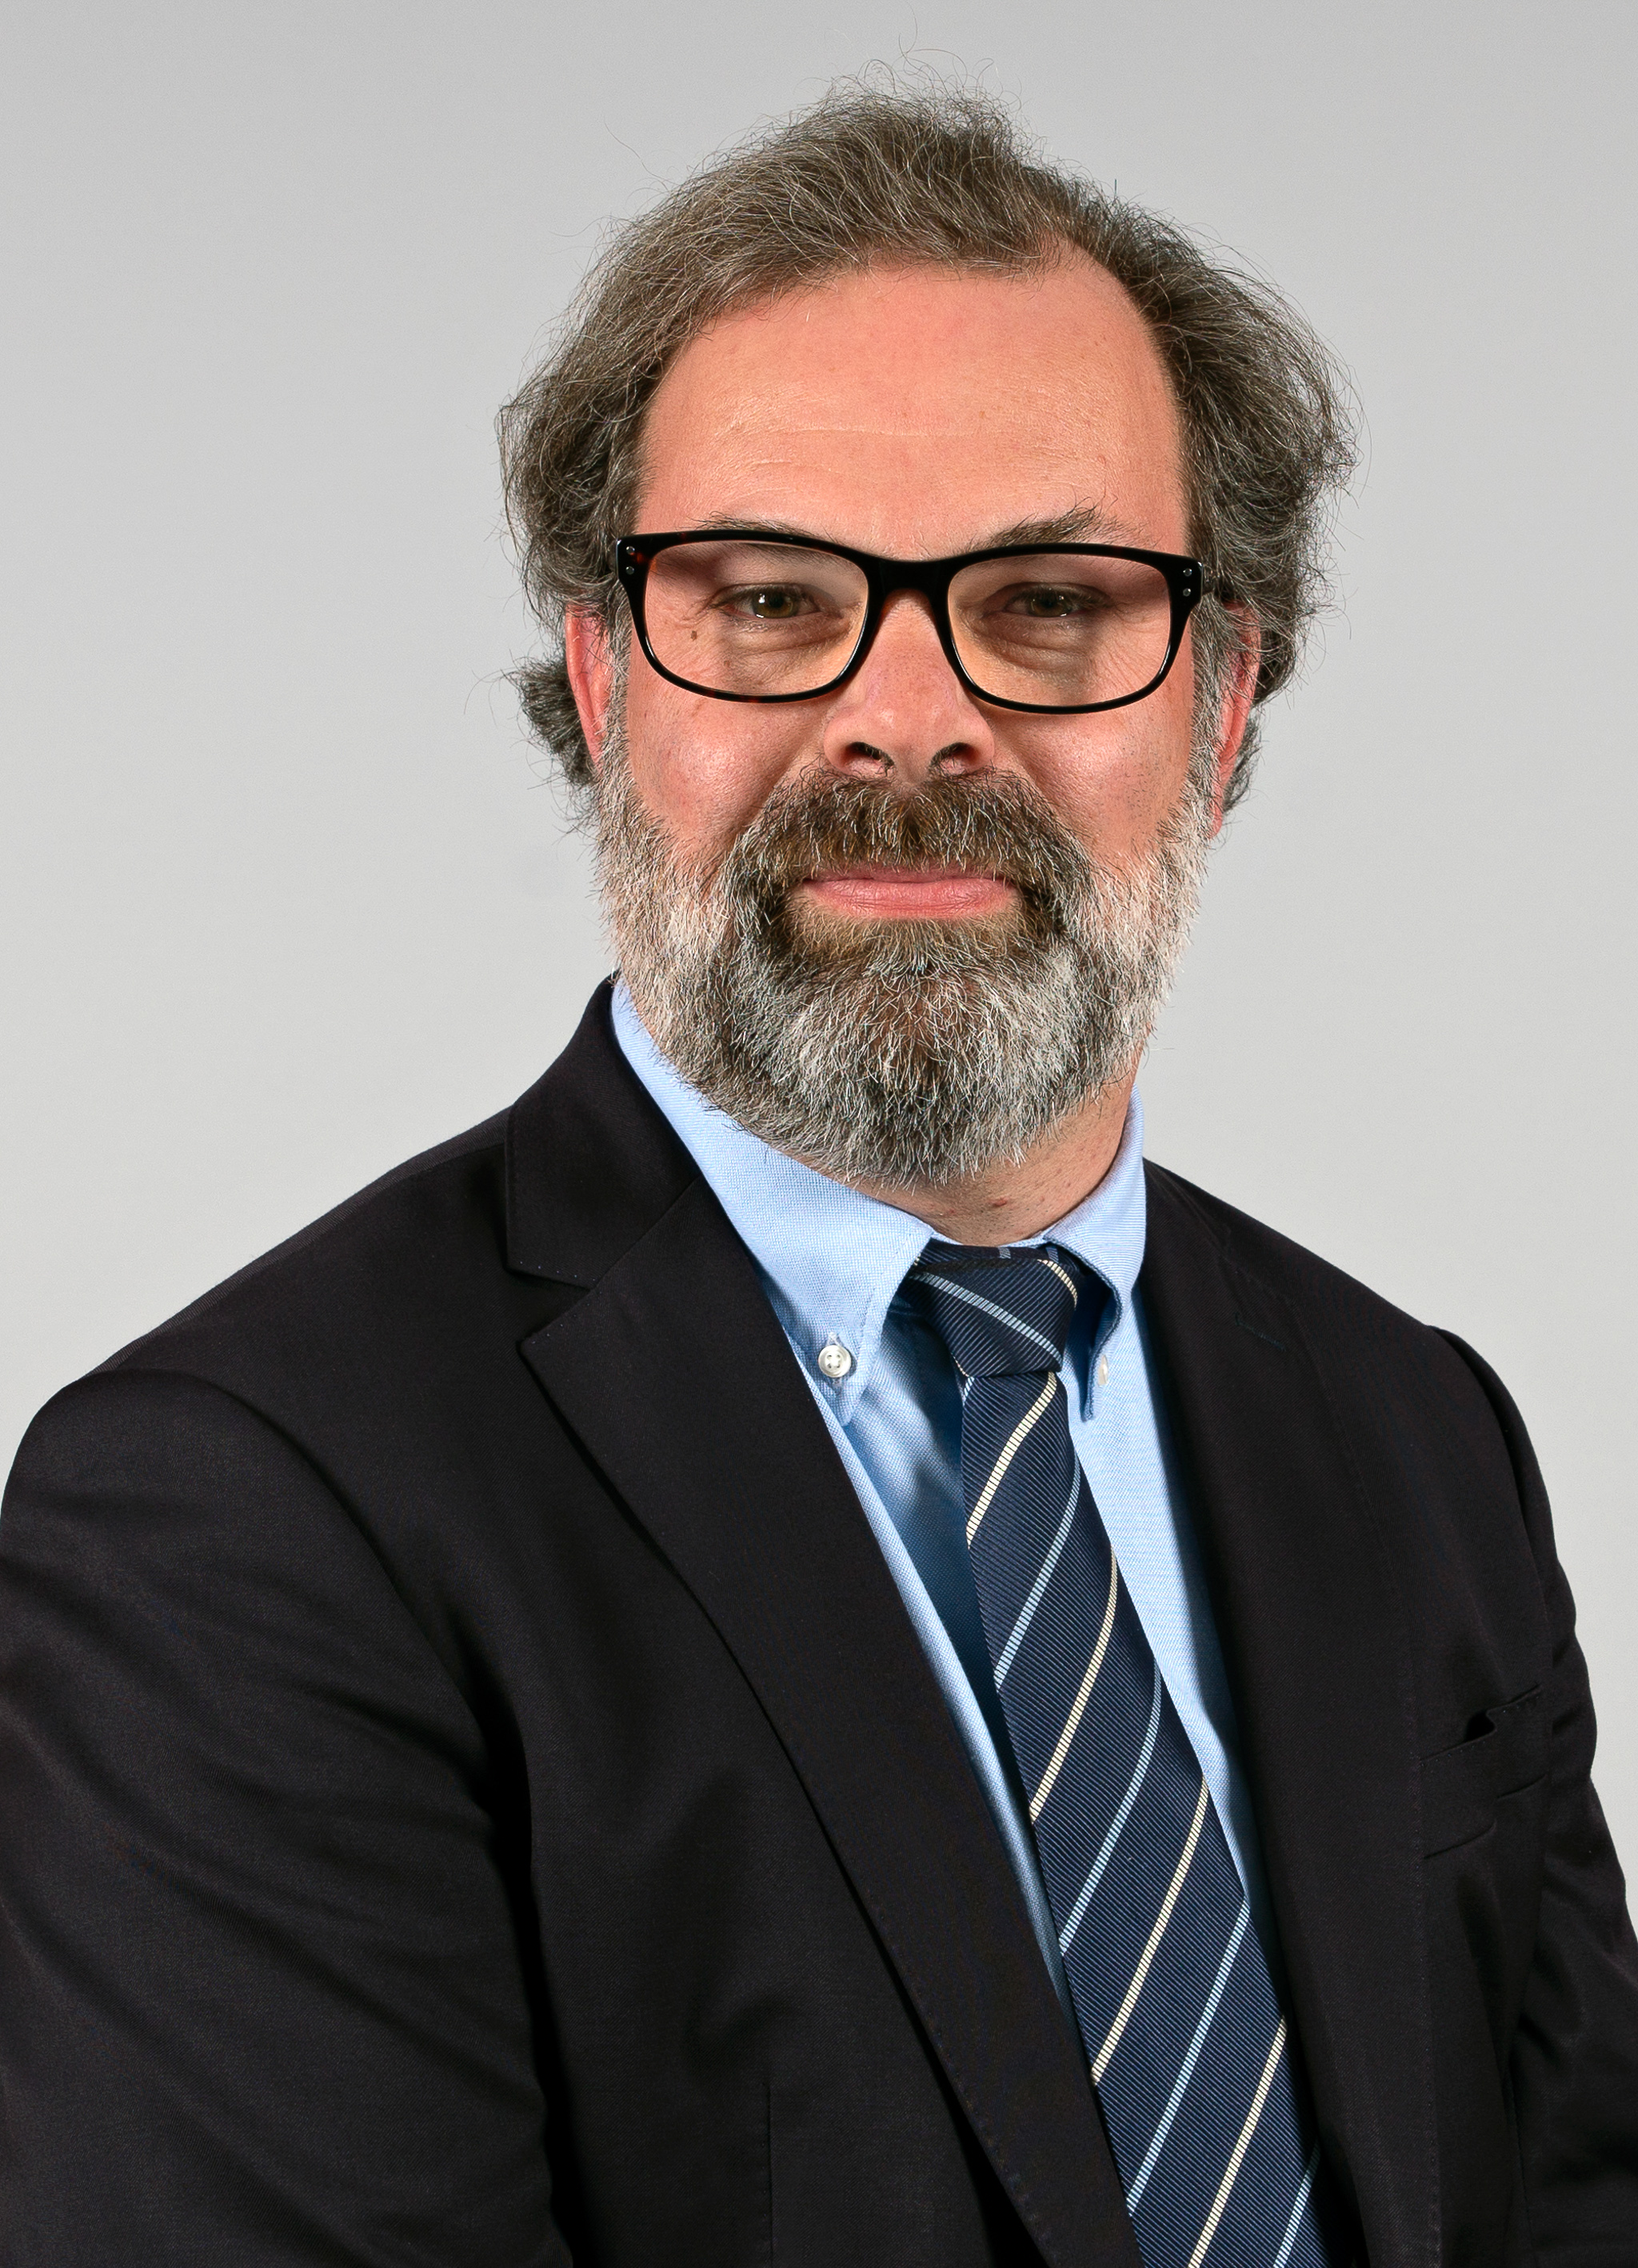
\includegraphics[width=0.9\linewidth]{images/elfaure.jpg}
        \caption{Bertrand Faure}
        \label{fig: 3}  
    \end{subfigure}
    \begin{subfigure}{0.4\textwidth}
        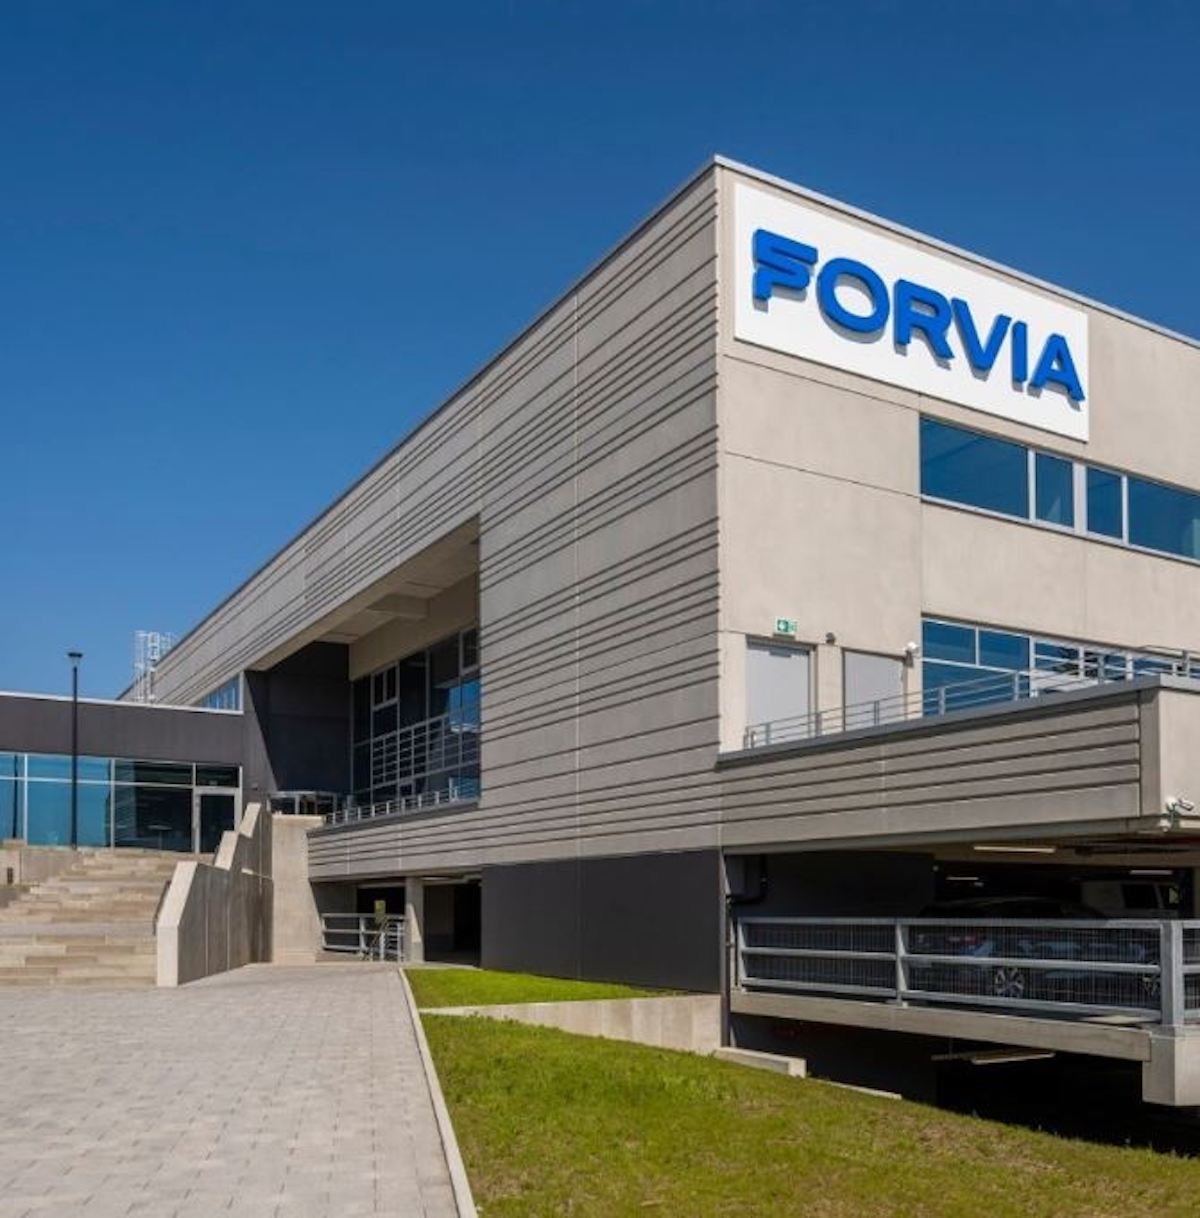
\includegraphics[width=0.9\linewidth]{images/ffffa.jpg}
        \caption{Forvia}
        \label{fig:4}
    \end{subfigure}
\end{figure}
\newpage
\begin{figure}[H]
    \centering
    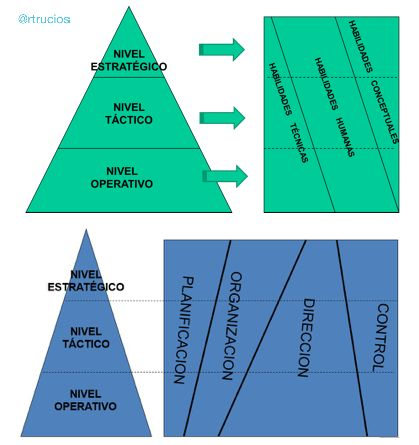
\includegraphics[width=0.6\textwidth]{images/niveles administrativos.jpg}
    \caption{Niveles Administrativos}
    \label{fig:5}
    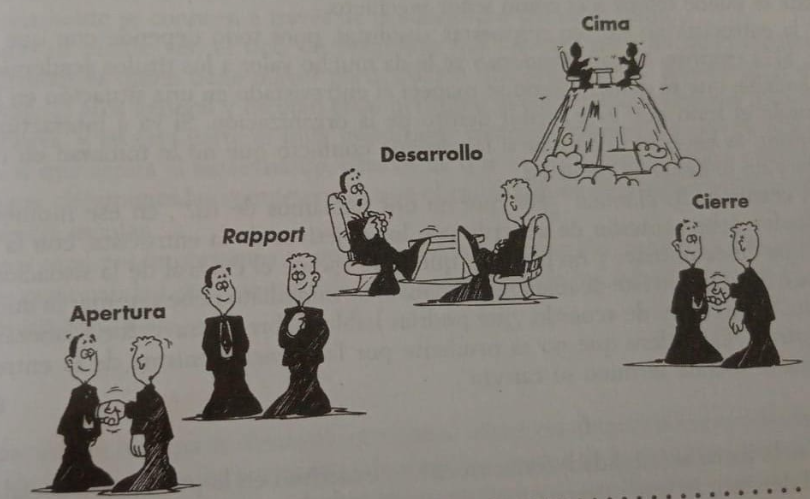
\includegraphics[width=0.4\textwidth]{images/entrevista.png}
    \caption{Proceso de entrevista colectiva}
    \label{fig:6}
    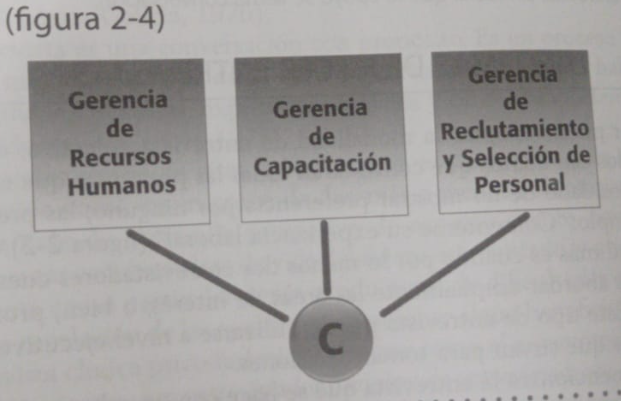
\includegraphics[width=0.4\textwidth]{images/entrevis2.png}
    \caption{Ejemplo de estructura de una entrevista empresarial}
    \label{fig:7}
\end{figure}
\newpage
\begin{figure}[H]
    \centering 
    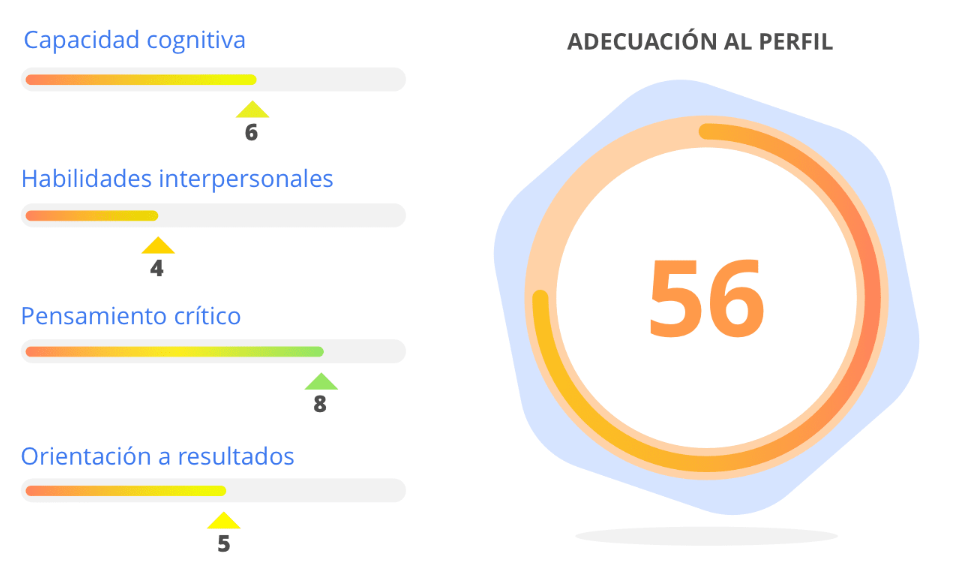
\includegraphics[width=0.8\textwidth]{images/ADECUACIONPER.png}
    \caption{Utilización del software bizneo y su objetividad sobre el perfil introducido}
\end{figure}


\end{sloppypar}
\end{document}

